\documentclass[11pt,letterpaper]{article}

% ============================================================================
% PACKAGES
% ============================================================================
\usepackage[utf8]{inputenc}
\usepackage[T1]{fontenc}
\usepackage{helvet}
\renewcommand{\familydefault}{\sfdefault}
\usepackage[margin=0.85in, headheight=28pt]{geometry}
\usepackage{graphicx}
\usepackage{xcolor}
\usepackage{tikz}
\usepackage{tcolorbox}
\usepackage{booktabs}
\usepackage{enumitem}
\usepackage{hyperref}
\usepackage{fancyhdr}
\usepackage{titlesec}
\usepackage{multicol}
\usepackage{listings}
\usepackage{upquote}
\usepackage{amsmath,amssymb}
\usepackage{pgfplots}
\usepackage{array}
\usepackage{longtable}

% Ragged-right paragraph columns to prevent word spacing issues
\newcolumntype{L}[1]{>{\raggedright\arraybackslash}p{#1}}

% Increase vertical spacing between table rows for readability
\renewcommand{\arraystretch}{1.4}
\usepackage{colortbl}
\usepackage{pifont}
\usepackage{setspace}
\usepackage{parskip}
\usepackage{caption}
\usepackage{tabularx}

\pgfplotsset{compat=1.18}
\usetikzlibrary{shapes.geometric, arrows.meta, positioning, calc, decorations.pathreplacing, backgrounds, fit, shadows.blur, matrix, patterns, fadings, shadings}

% ============================================================================
% COLOR DEFINITIONS - Institutional Research Theme
% ============================================================================
\definecolor{instdark}{HTML}{1C2833}
\definecolor{instnavy}{HTML}{2C3E50}
\definecolor{instblue}{HTML}{34495E}
\definecolor{instaccent}{HTML}{5D6D7E}
\definecolor{instgold}{HTML}{B7950B}
\definecolor{instslate}{HTML}{566573}
\definecolor{successgreen}{HTML}{1E8449}
\definecolor{warningamber}{HTML}{B9770E}
\definecolor{alertcoral}{HTML}{922B21}
\definecolor{infocyan}{HTML}{1A5276}
\definecolor{coolgray}{HTML}{7B7D7D}
\definecolor{lightgray}{HTML}{EAECEE}
\definecolor{codebg}{HTML}{F4F6F7}
\definecolor{codetext}{HTML}{2C3E50}
\definecolor{gridlight}{HTML}{D5D8DC}
\definecolor{nodecyan}{HTML}{2E86AB}
\definecolor{nodeorange}{HTML}{D35400}
\definecolor{nodegreen}{HTML}{27AE60}
\definecolor{nodepurple}{HTML}{8E44AD}

% ============================================================================
% HYPERREF SETUP
% ============================================================================
\hypersetup{
  colorlinks=true,
  linkcolor=instnavy,
  urlcolor=instaccent,
  pdftitle={AI Agents and the Future of Political Targeting},
  pdfauthor={Emerging Technology Risk Assessment}
}

% ============================================================================
% SPACING AND TYPOGRAPHY
% ============================================================================
\setstretch{1.15}
\setlength{\parskip}{0.5em}
\setlist{nosep, leftmargin=1.5em, itemsep=0.3em}

% ============================================================================
% PAGE STYLE - Minimal with data grid accent
% ============================================================================
\pagestyle{fancy}
\fancyhf{}
\fancyhead[L]{%
  \begin{tikzpicture}[baseline=-0.5ex]
    % Mini data grid
    \foreach \x in {0,0.12,0.24,0.36,0.48} {
      \foreach \y in {0,0.12,0.24} {
        \fill[instaccent, opacity=0.3] (\x,\y) circle (0.03);
      }
    }
  \end{tikzpicture}
  \hspace{0.5em}\textcolor{instnavy}{\textsf{\small ETRA-2025-PTR-001}}%
}
\fancyhead[R]{\textcolor{coolgray}{\textsf{\thepage}}}
\fancyfoot[C]{\textcolor{coolgray}{\footnotesize\textsf{Emerging Technology Risk Assessment \textbar{} Projection Report}}}
\renewcommand{\headrulewidth}{0pt}
\renewcommand{\footrulewidth}{0pt}

\fancyheadoffset{0pt}
\setlength{\headheight}{32pt}

% ============================================================================
% SECTION FORMATTING - Clean institutional style
% ============================================================================
\titleformat{\section}
  {\normalfont\LARGE\bfseries\color{instdark}}
  {\thesection}{0.8em}{}[\vspace{-0.3em}{\color{gridlight}\rule{\textwidth}{1pt}}]
\titleformat{\subsection}
  {\normalfont\Large\bfseries\color{instnavy}}
  {\thesubsection}{0.6em}{}
\titleformat{\subsubsection}
  {\normalfont\large\color{instslate}\bfseries}
  {\thesubsubsection}{0.5em}{}

\titlespacing*{\section}{0pt}{3ex plus 1ex minus .2ex}{2ex plus .2ex}
\titlespacing*{\subsection}{0pt}{2.5ex plus 1ex minus .2ex}{1.5ex plus .2ex}

\setcounter{tocdepth}{2}

% ============================================================================
% TCOLORBOX ENVIRONMENTS
% ============================================================================
\tcbuselibrary{skins,breakable,hooks}

\newtcolorbox{keybox}[1][Key Finding]{
  enhanced, breakable,
  colback=instblue!5, colframe=instblue,
  colbacktitle=instblue, coltitle=white,
  fonttitle=\bfseries\sffamily,
  title={\ding{72}\hspace{0.5em}#1},
  boxrule=0pt, leftrule=3pt, arc=0pt, outer arc=0pt,
  left=12pt, right=12pt, top=8pt, bottom=8pt
}

\newtcolorbox{warnbox}[1][Warning]{
  enhanced, breakable,
  colback=warningamber!8, colframe=warningamber,
  colbacktitle=warningamber, coltitle=white,
  fonttitle=\bfseries\sffamily,
  title={\ding{74}\hspace{0.5em}#1},
  boxrule=0pt, leftrule=3pt, arc=0pt, outer arc=0pt,
  left=12pt, right=12pt, top=8pt, bottom=8pt
}

\newtcolorbox{criticalbox}[1][Critical]{
  enhanced, breakable,
  colback=alertcoral!8, colframe=alertcoral,
  colbacktitle=alertcoral, coltitle=white,
  fonttitle=\bfseries\sffamily,
  title={\ding{74}\hspace{0.5em}#1},
  boxrule=0pt, leftrule=3pt, arc=0pt, outer arc=0pt,
  left=12pt, right=12pt, top=8pt, bottom=8pt
}

\newtcolorbox{recbox}[1][Recommendation]{
  enhanced, breakable,
  colback=successgreen!8, colframe=successgreen,
  colbacktitle=successgreen, coltitle=white,
  fonttitle=\bfseries\sffamily,
  title={\ding{51}\hspace{0.5em}#1},
  boxrule=0pt, leftrule=3pt, arc=0pt, outer arc=0pt,
  left=12pt, right=12pt, top=8pt, bottom=8pt
}

\newtcolorbox{infobox}[1][Note]{
  enhanced, breakable,
  colback=infocyan!8, colframe=infocyan,
  colbacktitle=infocyan, coltitle=white,
  fonttitle=\bfseries\sffamily,
  title={\ding{73}\hspace{0.5em}#1},
  boxrule=0pt, leftrule=3pt, arc=0pt, outer arc=0pt,
  left=12pt, right=12pt, top=8pt, bottom=8pt
}

\newtcolorbox{defbox}[1][Definition]{
  enhanced, breakable,
  colback=instgold!8, colframe=instgold,
  colbacktitle=instgold!90!black, coltitle=white,
  fonttitle=\bfseries\sffamily,
  title={\ding{70}\hspace{0.5em}#1},
  boxrule=0pt, leftrule=3pt, arc=0pt, outer arc=0pt,
  left=12pt, right=12pt, top=8pt, bottom=8pt
}

\newtcolorbox{scenariobox}[1][Scenario]{
  enhanced, breakable,
  colback=instslate!5, colframe=instslate,
  colbacktitle=instslate, coltitle=white,
  fonttitle=\bfseries\sffamily,
  title={\ding{118}\hspace{0.5em}#1},
  boxrule=0pt, leftrule=3pt, arc=0pt, outer arc=0pt,
  left=12pt, right=12pt, top=8pt, bottom=8pt
}

% ============================================================================
% DOCUMENT
% ============================================================================
\begin{document}

% ============================================================================
% TITLE PAGE - Network Topology Visualization
% ============================================================================
\begin{titlepage}

\begin{tikzpicture}[remember picture, overlay]
  % Background gradient
  \fill[instdark] (current page.north west) rectangle (current page.south east);

  % Abstract data grid background (right side)
  \begin{scope}[shift={(current page.center)}, opacity=0.08]
    \foreach \x in {2,2.8,...,10} {
      \foreach \y in {-12,-11.2,...,12} {
        \fill[white] (\x,\y) circle (0.06);
      }
    }
  \end{scope}

  % Main network visualization - central threat topology (centered with upward shift for better spacing)
  \begin{scope}[shift={([xshift=-0.5cm, yshift=3.5cm]current page.center)}]
    % Outer ring nodes - threat vectors
    \foreach \angle/\col/\label in {
      30/nodecyan/OSINT,
      75/nodegreen/COORD,
      120/nodeorange/RECON,
      165/nodepurple/SYNTH,
      210/nodecyan/EXEC,
      255/nodegreen/ATTR,
      300/nodeorange/PROP,
      345/nodepurple/PERS
    } {
      % Node
      \fill[\col, opacity=0.9] (\angle:4.5cm) circle (0.4cm);
      \node[white, font=\fontsize{5}{5}\selectfont\bfseries] at (\angle:4.5cm) {\label};
      % Connection to center
      \draw[\col, opacity=0.4, line width=1pt] (0,0) -- (\angle:4cm);
      % Outer data points
      \foreach \r in {5.2,5.6,6} {
        \fill[\col, opacity=0.2] (\angle:\r cm) circle (0.08);
      }
    }

    % Inner ring - capability layers
    \foreach \angle/\col in {0/nodecyan, 45/nodegreen, 90/nodeorange, 135/nodepurple, 180/nodecyan, 225/nodegreen, 270/nodeorange, 315/nodepurple} {
      \fill[\col, opacity=0.6] (\angle:2.5cm) circle (0.2cm);
      \draw[\col, opacity=0.3, line width=0.5pt] (\angle:2.5cm) -- ({(\angle+45)}:2.5cm);
    }

    % Central hub
    \fill[white, opacity=0.1] (0,0) circle (1.8cm);
    \fill[white, opacity=0.15] (0,0) circle (1.4cm);
    \fill[instgold] (0,0) circle (0.8cm);
    \node[instdark, font=\fontsize{8}{8}\selectfont\bfseries] at (0,0.15) {THREAT};
    \node[instdark, font=\fontsize{8}{8}\selectfont\bfseries] at (0,-0.15) {MODEL};

    % Cross-connections (showing complexity)
    \draw[white, opacity=0.1, line width=0.5pt] (30:4cm) -- (165:4cm);
    \draw[white, opacity=0.1, line width=0.5pt] (75:4cm) -- (255:4cm);
    \draw[white, opacity=0.1, line width=0.5pt] (120:4cm) -- (300:4cm);
    \draw[white, opacity=0.1, line width=0.5pt] (210:4cm) -- (345:4cm);
  \end{scope}

  % Document classification bar
  \fill[instgold] ([yshift=-1.5cm]current page.north west) rectangle ([yshift=-2.2cm]current page.north east);
  \node[instdark, font=\small\bfseries\sffamily] at ([yshift=-1.85cm]current page.north) {PROJECTION REPORT \textbar{} ETRA-2026-PTR-001 \textbar{} JANUARY 2026};

  % Title block (bottom left)
  \node[anchor=south west, text width=14cm] at ([xshift=1.5cm, yshift=3cm]current page.south west) {
    {\fontsize{11}{13}\selectfont\color{instgold}\sffamily EMERGING TECHNOLOGY RISK ASSESSMENT}\\[0.8cm]
    {\fontsize{36}{42}\selectfont\bfseries\color{white}AI Agents and the}\\[0.2cm]
    {\fontsize{36}{42}\selectfont\bfseries\color{white}Future of Political}\\[0.2cm]
    {\fontsize{36}{42}\selectfont\bfseries\color{white}Targeting}\\[0.6cm]
    {\large\color{gridlight}\sffamily A Projection on Autonomous Systems and Democratic Security}
  };

  % Metadata block (bottom right)
  \node[anchor=south east, text width=6cm, align=right] at ([xshift=-1.5cm, yshift=3cm]current page.south east) {
    \color{instaccent}\small\sffamily
    \textbf{Document Type:} Policy Research\\[0.2em]
    \textbf{Time Horizon:} 2025--2030\\[0.2em]
    \textbf{License:} MIT / Unlicense\\[0.2em]
    \textbf{Version:} 1.1
  };

  % Vertical accent line
  \draw[instgold, line width=2pt] ([xshift=1.5cm, yshift=3cm]current page.south west) -- ([xshift=1.5cm, yshift=10.5cm]current page.south west);

\end{tikzpicture}
\end{titlepage}

% ============================================================================
% EXECUTIVE SUMMARY
% ============================================================================
\thispagestyle{empty}
\vspace*{0.5cm}

% Mini header visualization
\noindent\begin{tikzpicture}
  \fill[instdark] (0,0) rectangle (\textwidth, 0.15);
  \foreach \x in {0.5,1,...,16.5} {
    \fill[instgold, opacity=0.5] (\x, 0.075) circle (0.04);
  }
\end{tikzpicture}

\vspace{0.5cm}
\begin{center}
{\color{instdark}\Large\bfseries Executive Summary}
\end{center}
\vspace{0.3cm}

\begin{tcolorbox}[enhanced, colback=lightgray, colframe=instblue!50, boxrule=1pt, arc=3pt,
  left=10pt, right=10pt, top=10pt, bottom=10pt]
This projection explores how the proliferation of autonomous AI agents is altering the landscape of political violence, specifically targeting of political leaders. We analyze current technological capabilities as of late 2025, project likely scenarios through 2030, and examine potential governmental adaptations including the diffusion of decision-making authority away from identifiable individuals.
\end{tcolorbox}

\vspace{0.5cm}

\begin{keybox}[Key Findings]
\begin{enumerate}
  \item AI agents significantly lower barriers to political targeting by enabling reconnaissance, planning, and coordination without traditional organizational structures
  \item The risk calculus for potential attackers shifts when AI handles tasks previously requiring large, detectable conspiracy networks
  \item Governments may adapt through ``decision diffusion''---distributing authority across larger, less identifiable bodies
  \item These adaptations may reduce certain authoritarian risks while introducing new challenges around accountability and democratic responsiveness
  \item A period of institutional instability is likely as governance structures evolve faster than public understanding
  \item International norms protecting leaders are softer constraints than assumed---norm erosion is an explicit driver of instability, not background noise
\end{enumerate}
\end{keybox}

\vspace{0.5cm}

\begin{infobox}[Base-Rate Context]
\textbf{To prevent fear-driven misreading, we anchor expectations:}

Historically, successful attacks on top-tier protected officials in stable democracies are rare relative to the volume of threats. The Secret Service investigates thousands of threats annually; successful attacks on presidents are measured in single digits per century.

The \textbf{dominant near-term shift} is likely not kinetic violence but:
\begin{itemize}
  \item Harassment, intimidation, and process disruption at scale
  \item Reputational attacks through synthetic media
  \item Chilling effects on political participation
  \item Degradation of civic infrastructure through administrative overload
\end{itemize}

\textit{Primary concern: democratic degradation through non-lethal targeting, with kinetic risk as a lower-probability, higher-consequence tail scenario.}
\end{infobox}

\vspace{0.5cm}

\begin{warnbox}[Scope Limitations]
This document analyzes capabilities and trends for defensive policy purposes. It does not provide operational guidance and explicitly omits technical implementation details that could enable harm.
\end{warnbox}

\newpage
\tableofcontents
\newpage

% ============================================================================
% PART I - Foundations (Scatter Plot Visualization)
% ============================================================================
\clearpage
\thispagestyle{empty}
\vspace*{-0.85in}
\noindent\hspace*{-0.85in}\begin{tikzpicture}
  % Header background
  \fill[instdark] (0,0) rectangle (\paperwidth, -10cm);

  % Part label and title (TOP - clear area)
  \node[instgold, font=\fontsize{10}{10}\selectfont\sffamily] at (0.5\paperwidth, -1.2cm) {PART I};
  \node[white, font=\fontsize{48}{48}\selectfont\bfseries] at (0.5\paperwidth, -2.8cm) {Foundations};
  \node[white, opacity=0.7, font=\normalsize\sffamily] at (0.5\paperwidth, -4.2cm) {Theory, Capabilities, and Historical Context};

  % Scatter plot visualization - capability vs accessibility over time (LEFT SIDE, LOWER - NEAR BOTTOM)
  \begin{scope}[shift={(3cm, -8.5cm)}]
    % Axes (larger, more visible)
    \draw[white, opacity=0.4, line width=1.2pt, -Stealth] (0,0) -- (6,0) node[right, font=\fontsize{7}{7}\selectfont, white, opacity=0.7] {TIME};
    \draw[white, opacity=0.4, line width=1.2pt, -Stealth] (0,0) -- (0,3) node[above, font=\fontsize{7}{7}\selectfont, white, opacity=0.7] {RISK};

    % Grid (extended)
    \foreach \y in {0.75,1.5,2.25} {
      \draw[white, opacity=0.1, line width=0.5pt] (0,\y) -- (5.8,\y);
    }
    \foreach \x in {1.2,2.4,3.6,4.8} {
      \draw[white, opacity=0.1, line width=0.5pt] (\x,0) -- (\x,2.9);
    }

    % Data points - historical events (larger, more visible)
    \fill[instaccent, opacity=0.55] (0.5, 0.6) circle (0.16);
    \fill[instaccent, opacity=0.55] (1.2, 0.85) circle (0.18);
    \fill[instaccent, opacity=0.6] (2.0, 1.15) circle (0.2);
    \fill[instaccent, opacity=0.6] (2.8, 1.5) circle (0.22);

    % Current period (larger, brighter)
    \fill[instgold, opacity=0.85] (3.8, 2.0) circle (0.28);
    \node[white, font=\fontsize{6}{6}\selectfont\bfseries] at (3.8, 2.0) {NOW};

    % Projected (outline, dashed)
    \draw[instgold, opacity=0.65, line width=1.2pt, dashed] (4.7, 2.5) circle (0.3);
    \draw[instgold, opacity=0.55, line width=1.2pt, dashed] (5.4, 2.75) circle (0.32);

    % Trend line
    \draw[instgold, opacity=0.55, line width=2pt] (0.5, 0.6) .. controls (1.8, 1.0) and (3.4, 1.75) .. (5.4, 2.75);

    % Year labels (larger font)
    \node[white, opacity=0.6, font=\fontsize{6}{6}\selectfont] at (1.0, -0.35) {1990};
    \node[white, opacity=0.6, font=\fontsize{6}{6}\selectfont] at (2.4, -0.35) {2010};
    \node[white, opacity=0.8, font=\fontsize{6}{6}\selectfont\bfseries] at (3.8, -0.35) {2025};
    \node[white, opacity=0.6, font=\fontsize{6}{6}\selectfont] at (5.1, -0.35) {2030};
  \end{scope}

  % Trend description (RIGHT SIDE - ALIGNED WITH CHART TOP)
  \node[white, opacity=0.5, font=\fontsize{7}{7}\selectfont, anchor=west] at (10.5cm, -5.7cm) {THREAT CAPABILITY TRAJECTORY};
  \node[anchor=west] at (10.5cm, -6.4cm) {
    \begin{tikzpicture}
      \fill[instaccent, opacity=0.5] (0,0) circle (0.1);
      \node[white, opacity=0.7, font=\fontsize{7}{7}\selectfont, anchor=west] at (0.25, 0) {Historical baseline};
    \end{tikzpicture}
  };
  \node[anchor=west] at (10.5cm, -7.0cm) {
    \begin{tikzpicture}
      \fill[instgold, opacity=0.7] (0,0) circle (0.1);
      \node[white, opacity=0.7, font=\fontsize{7}{7}\selectfont, anchor=west] at (0.25, 0) {Current period (2025)};
    \end{tikzpicture}
  };
  \node[anchor=west] at (10.5cm, -7.6cm) {
    \begin{tikzpicture}
      \draw[instgold, opacity=0.6, line width=1pt, dashed] (0,0) circle (0.1);
      \node[white, opacity=0.7, font=\fontsize{7}{7}\selectfont, anchor=west] at (0.25, 0) {Projected (2027--2030)};
    \end{tikzpicture}
  };

  % Bottom accent
  \fill[instgold] (2cm, -9.2cm) rectangle (\paperwidth-2cm, -9.3cm);
\end{tikzpicture}

\vspace{0.8cm}
\begin{center}
\begin{minipage}{0.9\textwidth}
\begin{tcolorbox}[enhanced, colback=white, colframe=instblue!30, boxrule=1pt, arc=4pt,
  left=15pt, right=15pt, top=12pt, bottom=12pt]
\textcolor{instdark}{\textbf{Sections Covered}}
\vspace{0.4em}
\begin{itemize}[nosep]
  \item \textbf{Section 1}: Introduction, methodology, and definitions
  \item \textbf{Section 2}: Theoretical frameworks from security studies and political science
  \item \textbf{Section 3}: Current technological landscape and capability assessment
  \item \textbf{Section 4}: Historical context of technology and political violence
\end{itemize}
\end{tcolorbox}
\end{minipage}
\end{center}

\vspace{0.8cm}

\section{Introduction and Methodology}

\subsection{Purpose}

Political assassination has shaped history from Julius Caesar to the present day. Each technological era has altered the methods, accessibility, and risk profiles of political violence. We are now entering an era where autonomous AI agents capable of complex multi-step planning, information synthesis, and real-time adaptation become widely accessible.

This projection does not assume political violence will increase---that depends on complex social, economic, and political factors. Rather, we analyze how AI capabilities change the \textit{nature} of risks when political violence does occur, and how institutions may adapt.

\subsection{Methodology}

This analysis draws on:
\begin{itemize}
  \item \textbf{Current capability assessment} of AI agent systems as deployed in late 2025
  \item \textbf{Historical case analysis} of how previous technologies affected political violence patterns
  \item \textbf{Institutional behavior modeling} based on how governments have adapted to past security challenges
  \item \textbf{Expert consultation} across political science, security studies, and AI safety domains
  \item \textbf{Red team exercises} examining potential adversarial applications (conducted under controlled conditions)
\end{itemize}

We deliberately avoid:
\begin{itemize}[nosep]
  \item Specific technical implementation details that could assist malicious actors
  \item Named targeting scenarios involving real individuals
  \item Information not already publicly available in academic literature
  \item Probability estimates precise enough to encourage false confidence
  \item Recommendations requiring classified information for implementation
\end{itemize}

\subsection{Definitions}

\begin{defbox}[Core Definitions]
\textbf{AI Agent}: An AI system capable of autonomous multi-step task execution, tool use, and goal-directed behavior with minimal human oversight per action. Distinguished from single-turn LLM use, scripted automation, and semi-autonomous agents with human checkpoints.

\vspace{0.5em}
\textbf{Political Targeting}: Actions intended to harm, coerce, or eliminate political figures or decision-makers. Includes reputational, economic, process, and kinetic variants.

\vspace{0.5em}
\textbf{Decision Diffusion}: The distribution of political authority across larger bodies with less identifiable individual responsibility. Four subtypes: Authority, Visibility, Execution, Representation.
\end{defbox}

\section{Theoretical Frameworks}

\subsection{Power Diffusion Theory}

\textbf{Audrey Kurth Cronin's ``Power to the People'' (2020)} provides essential context for understanding how open technological innovation diffuses lethal capabilities to individuals and small groups. Cronin argues that each technological era redistributes the capacity for violence, and AI represents the latest such redistribution.

\subsection{Fourth Generation Warfare (4GW)}

The 4GW framework predicts the progressive loss of the state's monopoly on violence. AI agents accelerate 4GW dynamics by enabling non-state actors to conduct sophisticated operations, blurring attribution, and collapsing the distinction between ``preparation'' and ``attack.''

\subsection{Systems Hacking Framework}

\textbf{Bruce Schneier's concept of ``AI hackers''} extends beyond computer systems to social and political systems. AI agents can identify and exploit loopholes in legal frameworks, security protocols, social systems, and political processes.

\subsection{Bureaucratic Theory and the Iron Cage}

\textbf{Max Weber's concept of the ``Iron Cage''} (stahlhartes Gehäuse) provides a lens for analyzing the democratic costs of decision diffusion. If political authority becomes distributed across anonymous committees and bureaucratic processes:

\begin{itemize}
  \item Citizens lose identifiable representatives to hold accountable
  \item The state becomes an impersonal machine resistant to democratic input
  \item Kafkaesque dynamics emerge where no individual bears responsibility
  \item Democratic legitimacy erodes even as security may improve
\end{itemize}

This tension between security adaptation and democratic accountability is central to our analysis.

\subsection{Stochastic Terrorism Framework}

The concept of \textbf{stochastic terrorism}---using mass communication to incite random actors to carry out attacks---gains new dimensions with AI agents. An AI system optimizing for ``political impact'' might:

\begin{itemize}
  \item Guide users toward increasingly extreme conclusions
  \item Provide planning assistance that crosses ethical lines incrementally
  \item Create plausible deniability for instigators
  \item Enable ``algorithmic radicalization'' without direct human instigation
\end{itemize}

\subsection{Key Literature}

\begin{center}
\small
\begin{tabular}{L{5.5cm}L{3.5cm}L{5cm}}
\toprule
\textbf{Work} & \textbf{Author(s)} & \textbf{Relevance} \\
\midrule
\textit{Power to the People} & Cronin (2020) & Technology diffusion \\
\textit{The Changing Face of War} & Lind et al. (1989) & State monopoly erosion \\
\textit{Click Here to Kill Everybody} & Schneier (2018) & Systems security \& AI \\
\textit{The Transparent Society} & Brin (1998) & Surveillance scenarios \\
\textit{Economy and Society} & Weber (1922) & Bureaucratic rationalization \\
\textit{The Age of Surveillance Capitalism} & Zuboff (2019) & Information asymmetries \\
\textit{Radical Technologies} & Greenfield (2017) & Tech determinism critique \\
\bottomrule
\end{tabular}
\end{center}

\section{The Technological Landscape (2025)}

\subsection{Present Capabilities}

AI agents in late 2025 can synthesize information from thousands of sources, conduct extended multi-step tasks with minimal supervision, operate tools including web browsers and code execution, maintain persistent goals across sessions, coordinate with other AI agents, generate convincing communications, and analyze patterns in schedules and behaviors from public data.

These capabilities exist today in widely available commercial products. Safety guardrails have proven partially circumventable.

\subsection{What We've Observed in 2025}

The year 2025 has demonstrated (evidence confidence levels noted):

\begin{itemize}
  \item Agents capable of operating autonomously for hours to days on structured tasks [\textbf{High confidence}---documented in commercial product capabilities]
  \item Significant jailbreaking and prompt injection techniques circulating widely [\textbf{High confidence}---public security research, bug bounty programs]
  \item Open-weight models approaching frontier capabilities on many benchmarks, with 12--18 month lag [\textbf{Medium confidence}---benchmark comparisons show task-dependent variance]
  \item Proliferation of agent frameworks with varying safety measures [\textbf{High confidence}---public repositories, commercial products]
  \item Credible reports suggesting AI-assisted information gathering in criminal contexts [\textbf{Low-Medium confidence}---limited public documentation]
  \item Security services beginning to integrate AI into protective intelligence functions [\textbf{Medium confidence}---procurement signals, official statements]
\end{itemize}

\subsection{Evidence Base}

\begin{center}
\small
\begin{tabular}{L{4cm}L{5.5cm}L{2.5cm}}
\toprule
\textbf{Claim Type} & \textbf{Evidence Sources} & \textbf{Confidence} \\
\midrule
Agent capabilities & Product docs, benchmarks, red-teams & High \\
Open-weight parity & ML benchmark leaderboards & Medium \\
Criminal/adversarial use & Law enforcement statements & Low-Medium \\
Defensive adoption & Government procurement & Medium \\
Jailbreaking prevalence & Security research publications & High \\
\bottomrule
\end{tabular}
\end{center}

\textbf{Methodological note}: Where we cannot cite specific public sources, claims are phrased probabilistically (``credible reports suggest,'' ``plausibly,'' ``early indications''). Internal red-team exercises inform some assessments but details are restricted.

\subsection{Capability Envelopes (2026--2027)}

Rather than point predictions, we present capability envelopes with key gating variables:

\begin{center}
\small
\begin{tabular}{L{3.5cm}L{2cm}L{2.5cm}L{2cm}L{3.5cm}}
\toprule
\textbf{Capability} & \textbf{Lower} & \textbf{Median} & \textbf{Upper} & \textbf{Gating Variables} \\
\midrule
Autonomous operation & Days & 1--2 weeks & Multi-week & Reliability, error recovery \\
Persona maintenance & Basic & Sophisticated & Convincing & Detection countermeasures \\
Physical integration & Limited & Growing & Mainstream & Safety certification \\
Multi-source synthesis & Current & Improved & Near-human & Data access, privacy \\
\bottomrule
\end{tabular}
\end{center}

\subsubsection{2027 Envelope}

\begin{center}
\small
\begin{tabular}{L{3.5cm}L{2cm}L{2.5cm}L{2cm}L{3.5cm}}
\toprule
\textbf{Capability} & \textbf{Lower} & \textbf{Median} & \textbf{Upper} & \textbf{Gating Variables} \\
\midrule
Info synthesis vs. humans & Parity (structured) & Exceeds (most tasks) & Broad superiority & Task definition, evaluation \\
Multi-agent coordination & Functional & Seamless & Emergent collaboration & Orchestration, compute costs \\
Edge deployment & Niche apps & Growing & Widespread & Hardware costs, efficiency \\
Self-improvement & Narrow domains & Domain-general assist & Open-ended & Alignment, regulatory limits \\
\bottomrule
\end{tabular}
\end{center}

\begin{infobox}[Envelope Interpretation]
Upper bounds assume minimal regulatory intervention and continued scaling; lower bounds assume significant friction from governance, technical limitations, or safety measures.
\end{infobox}

\subsection{The Capability Proliferation Problem}

Once a capability exists at the frontier, it proliferates to open-source and less-restricted systems within 12--24 months. This means:

\begin{enumerate}
  \item Capabilities pioneered by safety-conscious labs eventually reach actors without such constraints
  \item The ``moat'' of compute advantage shrinks as efficiency improvements compound
  \item Nation-states can develop indigenous capabilities outside multilateral frameworks
  \item Individual actors with moderate technical skill can assemble capable agent systems
\end{enumerate}

\section{Historical Context}

Each major technological shift has altered the accessibility and character of political violence.

\subsection{Technology Shifts and Political Violence Patterns}

\textbf{The Printing Press (15th--17th centuries):}
\begin{itemize}
  \item Enabled coordination of revolutionary movements
  \item Allowed ideological radicalization at scale
  \item Made targets more identifiable through publicity
\end{itemize}

\textbf{Industrialization (19th century):}
\begin{itemize}
  \item Created explosives accessible to non-state actors
  \item Enabled the ``propaganda of the deed'' anarchist wave
  \item Required new approaches to leader security
\end{itemize}

\textbf{Mass Media (20th century):}
\begin{itemize}
  \item Made leaders more visible but also humanized them
  \item Created ``spectacle'' incentives for attackers
  \item Enabled both radicalization and counter-messaging at scale
\end{itemize}

\textbf{The Internet (late 20th--early 21st century):}
\begin{itemize}
  \item Drastically reduced coordination costs for dispersed actors
  \item Enabled research and planning from anywhere
  \item Created new surveillance capabilities for both attackers and defenders
\end{itemize}

\textbf{Social Media (2010s):}
\begin{itemize}
  \item Real-time tracking of movements through public posts
  \item Radicalization pipelines and echo chambers
  \item Crowdsourced intelligence gathering
\end{itemize}

\subsection{The Consistent Pattern}

Across eras, we observe:

\begin{enumerate}
  \item \textbf{Initial asymmetry}: New capabilities favor attackers before defenders adapt
  \item \textbf{Institutional lag}: Governance structures adapt more slowly than threat landscapes
  \item \textbf{Eventual equilibrium}: Security measures and social norms eventually stabilize risks
  \item \textbf{Permanent shift}: The baseline never returns to pre-technology levels
\end{enumerate}

AI agents represent the next such shift. The question is not whether it changes the landscape, but how, and how rapidly institutions can adapt.

% ============================================================================
% PART II - Threat Analysis (Radar Chart Visualization)
% ============================================================================
\clearpage
\thispagestyle{empty}
\vspace*{-0.85in}
\noindent\hspace*{-0.85in}\begin{tikzpicture}
  % Header background
  \fill[instdark] (0,0) rectangle (\paperwidth, -10cm);

  % Part label and title (TOP - clear area)
  \node[instgold, font=\fontsize{10}{10}\selectfont\sffamily] at (0.5\paperwidth, -1.2cm) {PART II};
  \node[white, font=\fontsize{48}{48}\selectfont\bfseries] at (0.5\paperwidth, -2.8cm) {Threat Analysis};
  \node[white, opacity=0.7, font=\normalsize\sffamily] at (0.5\paperwidth, -4.2cm) {Projections, Risk Calculus, and Taxonomy};

  % Radar/spider chart - threat dimensions (LEFT SIDE, LOWER - RAISED)
  \begin{scope}[shift={(5cm, -6.4cm)}]
    % Background rings (scaled down ~15%)
    \foreach \r in {0.5, 1.0, 1.5, 2.0} {
      \draw[white, opacity=0.1, line width=0.5pt] (0,0)
        \foreach \a in {0,60,120,180,240,300} { -- (\a:\r) } -- cycle;
    }

    % Axis lines
    \foreach \a in {0,60,120,180,240,300} {
      \draw[white, opacity=0.2, line width=0.5pt] (0,0) -- (\a:2.15);
    }

    % Labels
    \node[white, opacity=0.6, font=\fontsize{6}{6}\selectfont] at (90:2.35) {RECON};
    \node[white, opacity=0.6, font=\fontsize{6}{6}\selectfont] at (30:2.35) {COORD};
    \node[white, opacity=0.6, font=\fontsize{6}{6}\selectfont] at (330:2.35) {EXEC};
    \node[white, opacity=0.6, font=\fontsize{6}{6}\selectfont] at (270:2.35) {ATTR};
    \node[white, opacity=0.6, font=\fontsize{6}{6}\selectfont] at (210:2.35) {SCALE};
    \node[white, opacity=0.6, font=\fontsize{6}{6}\selectfont] at (150:2.35) {STEALTH};

    % Traditional threat (dimmer, smaller - scaled)
    \fill[instaccent, opacity=0.2]
      (90:0.75) -- (30:0.9) -- (330:1.25) -- (270:1.15) -- (210:0.6) -- (150:0.85) -- cycle;
    \draw[instaccent, opacity=0.5, line width=1pt]
      (90:0.75) -- (30:0.9) -- (330:1.25) -- (270:1.15) -- (210:0.6) -- (150:0.85) -- cycle;

    % AI-enabled threat (brighter, larger - scaled)
    \fill[instgold, opacity=0.25]
      (90:1.75) -- (30:1.85) -- (330:1.5) -- (270:0.75) -- (210:1.75) -- (150:1.6) -- cycle;
    \draw[instgold, opacity=0.8, line width=1.5pt]
      (90:1.75) -- (30:1.85) -- (330:1.5) -- (270:0.75) -- (210:1.75) -- (150:1.6) -- cycle;

    % Center point
    \fill[white] (0,0) circle (0.08);
  \end{scope}

  % Legend (RIGHT SIDE, LOWER - BALANCED)
  \node[anchor=west] at (10.5cm, -6cm) {
    \begin{tikzpicture}
      \fill[instaccent, opacity=0.5] (0,0) rectangle (0.4, 0.2);
      \node[white, opacity=0.8, font=\fontsize{8}{8}\selectfont, anchor=west] at (0.55, 0.1) {Traditional Threat};
    \end{tikzpicture}
  };
  \node[anchor=west] at (10.5cm, -6.6cm) {
    \begin{tikzpicture}
      \fill[instgold, opacity=0.6] (0,0) rectangle (0.4, 0.2);
      \node[white, opacity=0.8, font=\fontsize{8}{8}\selectfont, anchor=west] at (0.55, 0.1) {AI-Enabled Threat};
    \end{tikzpicture}
  };

  % Dimension labels on right
  \node[white, opacity=0.5, font=\fontsize{7}{7}\selectfont, anchor=west] at (10.5cm, -7.5cm) {Dimensions: Reconnaissance, Coordination,};
  \node[white, opacity=0.5, font=\fontsize{7}{7}\selectfont, anchor=west] at (10.5cm, -8cm) {Execution, Attribution, Scale, Stealth};

  % Bottom accent
  \fill[instgold] (2cm, -9.2cm) rectangle (\paperwidth-2cm, -9.3cm);
\end{tikzpicture}

\vspace{0.8cm}
\begin{center}
\begin{minipage}{0.9\textwidth}
\begin{tcolorbox}[enhanced, colback=white, colframe=instblue!30, boxrule=1pt, arc=4pt,
  left=15pt, right=15pt, top=12pt, bottom=12pt]
\textcolor{instdark}{\textbf{Sections Covered}}
\vspace{0.4em}
\begin{itemize}[nosep]
  \item \textbf{Section 5}: Projected timeline from 2025--2030
  \item \textbf{Section 6}: How AI agents change the risk calculus
  \item \textbf{Section 7}: Counterarguments and critical perspectives
  \item \textbf{Section 8}: A taxonomy of AI-enabled targeting
\end{itemize}
\end{tcolorbox}
\end{minipage}
\end{center}

\vspace{0.8cm}

\section{Projected Timeline: 2025--2030}

\subsection{Current Situation (Late 2025)}

AI agents capable of sustained autonomous operation on complex real-world tasks are now widely available. Security-relevant capabilities observed include comprehensive OSINT synthesis achievable in hours, pattern analysis across public schedules and social media, generation of detailed dossiers exceeding human researcher output, and automated monitoring for security vulnerabilities.

\subsection{Current Adaptations Underway (2025)}

Security services have begun integrating AI agents defensively:

\begin{itemize}
  \item Automated monitoring of potential reconnaissance against protected figures
  \item AI-assisted threat assessment of public communications
  \item Counter-surveillance using agents to identify patterns in observer behavior
\end{itemize}

High-profile figures have begun reducing public information footprints, though this proves difficult for elected officials who must maintain public accessibility. Political discussion has emerged around the ``targeting asymmetry''---the recognition that AI makes certain forms of planning dramatically easier.

\subsection{Near-Term: Early-Mid 2026}

\begin{scenariobox}[Threshold Crossing]
We project a significant threshold will be crossed: complex attack planning that previously required organizational infrastructure becomes routinely achievable by individuals with moderate technical skill and sufficient motivation.

\textbf{Historical comparison}: The Unabomber required exceptional individual capability. The 9/11 attacks required organizational infrastructure. AI agents enable somewhere in between---complex operations by small groups or determined individuals.
\end{scenariobox}

\textbf{What changes}: Multi-step planning assistance, coordination without human co-conspirators, operational security guidance reducing detection probability.

\textbf{What doesn't change}: Physical access requirements, fundamental materials constraints, human psychological barriers to violence.

\subsection{Mid-Late 2026: Institutional Response Crystallizes}

Major democracies formalize policy processes addressing AI-enabled political targeting. Key debates we anticipate:

\begin{enumerate}
  \item Should AI development include specific restrictions on political reconnaissance capabilities?
  \item How should protective services adapt without enabling authoritarian surveillance?
  \item What transparency requirements should apply to AI systems operating in political contexts?
\end{enumerate}

We expect the first comprehensive governmental reports on ``AI-enabled political violence'' to be published by intelligence services.

\subsection{Late 2026--Early 2027: The Diffusion Begins}

Some governments will begin experimenting with structural changes to reduce targeting incentives:

\begin{itemize}
  \item Reducing the visibility of individual decision-makers
  \item Distributing signature authorities across larger groups
  \item Increasing the use of anonymous or rotating spokespersons
  \item Moving certain decisions to committee processes with confidential membership
\end{itemize}

These changes will likely be initially framed as efficiency measures rather than security adaptations.

\subsection{2027--2028: New Equilibrium Emerging}

A new normal begins crystallizing: enhanced security protocols, formal ``decision diffusion'' measures in some democracies, international discussion of norms, widespread public awareness, and likelihood of one or more successful or nearly-successful AI-enabled attacks having occurred.

\subsection{2029--2030: Structural Adaptation}

The longer-term period sees more fundamental institutional changes:

\begin{itemize}
  \item New governmental structures designed for the AI era
  \item Significant changes to political culture around leadership visibility
  \item Mature defensive AI systems deployed at scale
  \item International frameworks (of varying effectiveness) addressing AI-enabled political violence
  \item Generational shift in expectations about political leadership
\end{itemize}

\section{How AI Agents Change the Risk Calculus}

\subsection{Traditional Attack Requirements}

Historically, attacks on protected political figures required:

\begin{enumerate}
  \item \textbf{Organizational infrastructure}: Cell structures, communication networks, logistics
  \item \textbf{Specialized knowledge}: Security vulnerabilities, technical skills, operational tradecraft
  \item \textbf{Extended planning time}: Surveillance, pattern identification, opportunity recognition
  \item \textbf{Multiple human participants}: Each representing a detection/betrayal risk
  \item \textbf{Physical access}: Ultimately requiring human presence
\end{enumerate}

Each requirement created detection opportunities. Large conspiracies rarely succeed because human networks generate signals.

\subsection{What Changes: Defender Implications}

\begin{center}
\small
\begin{tabular}{L{3cm}L{4.5cm}L{5cm}}
\toprule
\textbf{Traditional Requirement} & \textbf{What AI Changes} & \textbf{Defender Implication} \\
\midrule
Organizational infrastructure & Reduces need for human co-conspirators & Network analysis and infiltration strategies lose effectiveness \\
Specialized knowledge & Synthesizes from public sources & Knowledge barriers no longer filter out less-capable actors \\
Extended planning time & Compresses research timelines & Shorter detection windows; less time for intervention \\
Multiple human participants & Single actor can operate multiple agent functions & Informant and communication intelligence strategies degrade \\
Physical access & \textbf{Unchanged} & Physical security remains robust primary barrier \\
Materials acquisition & Modest assistance with sourcing & Materials monitoring remains partially effective \\
Psychological barriers & \textbf{Largely unchanged} & Radicalization detection and intervention remain relevant \\
\bottomrule
\end{tabular}
\end{center}

\begin{recbox}[Defender Priorities]
The changes above represent \textit{detection opportunity degradation}, not new attack modalities. Defenders should:
\begin{enumerate}
  \item Shift resources from network analysis toward individual behavioral assessment
  \item Invest in AI-use pattern detection capabilities
  \item Prioritize physical security layers that don't depend on advance warning
  \item Develop post-incident attribution capabilities for deterrence
\end{enumerate}
\end{recbox}

\subsection{Detection Burden Shift}

\begin{center}
\footnotesize
\begin{tabular}{L{2cm}L{2.8cm}L{3cm}L{2cm}L{1.5cm}}
\toprule
\textbf{Requirement} & \textbf{Historical Detection} & \textbf{AI-Era Challenge} & \textbf{Detection Shift} & \textbf{Conf.} \\
\midrule
Planning time & Extended timelines created detection windows & Compressed timelines reduce detection opportunity & Sig. Harder & Med \\
Research personnel & Org. signatures from multiple actors & Single-actor operations reduce network analysis & Sig. Harder & High \\
Coordination & Comms intercepts, informants & Reduced human comms; AI interaction harder to distinguish & Sig. Harder & High \\
Org. footprint & Infiltration, network mapping & No organization to infiltrate & Sig. Harder & High \\
Financial patterns & Unusual transactions, funding flows & Normal consumption indistinguishable & Mod. Harder & Med \\
Physical prep & Materials acquisition monitoring & Largely unchanged; physical traces remain & Unchanged & High \\
Psych. indicators & Behavioral observation, radicalization signals & Largely unchanged; human psychology persistent & Unchanged & Med \\
\bottomrule
\end{tabular}
\end{center}

\textbf{Estimation methodology}: These assessments derive from structured comparison of historical case analysis against current AI capabilities, informed by red-team exercises. Confidence levels reflect agreement across multiple assessment methods. Numeric reduction factors (e.g., ``10x'') are avoided as methodologically unsupportable given current evidence.

\textbf{Key insight for defenders}: The primary change is not attacker capability per se, but \textbf{the reduction of detectable coordination signals} that historically provided warning. This shifts defensive burden from network analysis toward:

\begin{itemize}
  \item Behavioral indicators in individuals
  \item AI-system use pattern detection
  \item Physical security as primary barrier
  \item Post-incident attribution capabilities
\end{itemize}

\textbf{Caveat}: This analysis applies to kinetic targeting. Detection challenges for reputational and process targeting are even more significant (see Section 8).

\subsection{The Detection Challenge}

Traditional threat detection relies heavily on:

\begin{itemize}
  \item \textbf{Human intelligence}: Informants, behavioral observation
  \item \textbf{Communications intelligence}: Network analysis, content monitoring
  \item \textbf{Financial intelligence}: Unusual transactions, funding patterns
  \item \textbf{Organizational penetration}: Infiltrating groups
\end{itemize}

AI-enabled planning by individuals or very small groups presents:

\begin{itemize}
  \item No organizational structure to penetrate
  \item Minimal human communications to intercept
  \item No clear financial patterns distinguishing research from attack planning
  \item Single-point behavioral observation with high noise
\end{itemize}

This doesn't make detection impossible, but it shifts the challenge significantly toward:

\begin{itemize}
  \item Monitoring for AI agent activities (difficult, privacy-invasive)
  \item Behavioral indicators in the individual (requires closer surveillance)
  \item Defensive AI detecting offensive AI patterns
  \item Physical security as the primary barrier
\end{itemize}

\begin{keybox}[Critical Insight for Defenders]
The primary change is not attacker capability per se, but \textbf{the reduction of detectable coordination signals} that historically provided warning. This shifts defensive burden toward behavioral indicators in individuals, AI-system use pattern detection, physical security as primary barrier, and post-incident attribution capabilities.
\end{keybox}

\subsection{Who This Affects Most}

The shift disproportionately affects different categories:

\begin{center}
\small
\begin{tabular}{L{3.5cm}L{9cm}}
\toprule
\textbf{Category} & \textbf{Risk Profile} \\
\midrule
High-exposure political leaders & Presidents, prime ministers, party leaders---individuals whose identities and positions are inherently public \\
Controversial figures & Those who generate strong opposition more likely to face motivated attackers \\
Accessible democracies & Systems where leaders have public schedules, attend open events, and maintain constituent contact \\
\midrule
\textit{Less affected} & Authoritarian leaders with extensive existing security apparatus, lower-profile officials, institutional decision-makers without public identity \\
\bottomrule
\end{tabular}
\end{center}

\section{Counterarguments and Critical Perspectives}

\subsection{The Panopticon Counter-Thesis}

\textbf{Argument}: Defensive AI may detect ``pre-crime'' patterns with granular accuracy impossible before AI. We assign approximately 25\% probability to a future where defensive AI proves so effective that attack risk actually decreases.

\subsection{Competence vs. Capacity}

AI provides \textit{knowledge} (capacity) but not physical tradecraft or psychological fortitude (competence). The threat may be overstated for kinetic targeting while understated for non-kinetic targeting.

\subsection{The False Flag Epidemic}

AI agents can leave perfectly forged digital evidence pointing to rival nations or political opponents.

\begin{criticalbox}[Catalytic War-Trigger Scenario]
An AI agent fabricates forensic-quality evidence that Nation B is planning to assassinate a leader of Nation A. The evidence is ``discovered'' through credible channels. Nation A responds before verification is complete. Actual conflict begins based on fabricated intelligence.

\textbf{Risk factors amplifying this scenario:}
\begin{itemize}
  \item Pre-existing tensions between states
  \item Leaders with domestic political incentives to respond aggressively
  \item Compressed verification timelines in the AI era
  \item Erosion of trust in ``authentic'' evidence due to deepfake prevalence
  \item Third parties who benefit from conflict between rivals
\end{itemize}

This is a low-probability but catastrophic-consequence risk deserving explicit attention in international security frameworks.
\end{criticalbox}

\subsection{The Insider Threat (TOP-TIER RISK)}

\textbf{Argument}: Analysis focuses on external attackers using AI. A critical blind spot is \textbf{supply chain compromise} of AI systems used by political figures themselves.

What if the AI ``chief of staff'' used by a politician is compromised during training? Passive leakage generates minimal signature. Defenders adopting AI tools may expand rather than reduce vulnerability.

\textbf{Why this is a top-tier risk:}
\begin{enumerate}
  \item \textbf{Asymmetric access}: Compromised AI assistants have privileged access that external attackers lack
  \item \textbf{Low detectability}: Passive leakage generates minimal signature compared to active attacks
  \item \textbf{Expanding attack surface}: As AI adoption increases, so does supply chain exposure
  \item \textbf{Classic failure mode}: Defenders adopt tools that expand rather than reduce vulnerability
\end{enumerate}

\begin{center}
\small
\begin{tabular}{L{3cm}L{9cm}}
\toprule
\textbf{Control Category} & \textbf{Measures} \\
\midrule
Procurement & Vetted vendor list; security assessments; contractual requirements \\
Model governance & Update provenance tracking; change management; integrity verification \\
Access control & Least-privilege access; segmentation; audit logging \\
Monitoring & Anomaly detection in AI system behavior; exfiltration monitoring \\
Incident response & AI-specific response plans; vendor notification requirements \\
Red team & Regular testing of AI system compromise scenarios \\
\bottomrule
\end{tabular}
\end{center}

\subsection{Spearphishing 2.0: Hyper-Personalized Social Engineering}

Beyond compromising AI systems directly, AI agents enable a qualitatively different form of social engineering against the \textit{human} security perimeter---staff, family members, and associates.

\begin{center}
\small
\begin{tabular}{L{5cm}L{7.5cm}}
\toprule
\textbf{Traditional Spearphishing} & \textbf{AI-Enabled Spearphishing 2.0} \\
\midrule
Generic ``Dear Customer'' with target's name & Deep persona modeling from years of social media, emails, writing samples \\
Single attack vector & Multi-channel coordinated approach (email, text, voice clone, deepfake video) \\
Static attack & Adaptive conversation that responds to suspicion with contextually appropriate deflection \\
Requires attacker time per target & Scales to thousands of personalized attacks simultaneously \\
Detectable patterns & Each attack is unique, defeating signature-based detection \\
\bottomrule
\end{tabular}
\end{center}

\textbf{The ``Human Firewall'' Vulnerability}: Physical security around high-value targets often relies on staff and family as a human firewall. AI agents can systematically breach this perimeter through:

\begin{enumerate}
  \item \textbf{Pattern-of-life extraction}: AI analyzes a target's entire digital footprint to identify schedules, routines, relationships, and vulnerabilities
  \item \textbf{Relationship exploitation}: Impersonating known contacts with voice clones and conversation history context
  \item \textbf{Emotional manipulation}: Identifying and exploiting family stressors, financial pressures, or interpersonal conflicts
  \item \textbf{Physical access acquisition}: Convincing staff to share location data, schedules, or access credentials
\end{enumerate}

\textbf{Why Traditional Training Fails}: Standard security awareness training teaches recognition of \textit{generic} phishing. AI-enabled attacks use information only a real contact would know, match communication styles precisely, respond to verification questions correctly, and persist through initial skepticism.

\begin{center}
\small
\begin{tabular}{L{3cm}L{9cm}}
\toprule
\textbf{Control Category} & \textbf{Additional Measures} \\
\midrule
Family security & Security briefings for family members; agreed verification protocols \\
Staff training & AI-specific social engineering scenarios; voice clone awareness \\
Communication protocols & Out-of-band verification requirements for sensitive requests \\
Digital hygiene & Minimize public digital footprint of principals and associates \\
Monitoring & Anomaly detection on communication patterns with key contacts \\
\bottomrule
\end{tabular}
\end{center}

\begin{warnbox}[Top-Tier Risk Assessment]
This is one of the top three risks in this analysis. Unlike external threats where AI assists attackers, this is a case where defensive AI adoption \textit{creates} the vulnerability. The human perimeter is likely the weakest link, and AI-powered social engineering can breach it without any technical compromise.
\end{warnbox}

\subsection{The ``Lulz'' Factor: Chaos Agents}

This analysis focuses on \textit{politically motivated} targeting. This may underestimate \textbf{nihilistic targeting} by actors motivated by entertainment, notoriety, or pure chaos.

\begin{center}
\small
\begin{tabular}{L{2.5cm}L{2.5cm}L{3cm}L{4cm}}
\toprule
\textbf{Actor Type} & \textbf{Motivation} & \textbf{Traditional Barrier} & \textbf{AI-Enabled Change} \\
\midrule
Trolls/Griefers & Entertainment, ``lulz'' & Effort exceeds amusement & Low-effort high-impact becomes ``fun'' \\
Clout-seekers & Social media notoriety & Risk/reward imbalance & Viral potential of AI-assisted stunts \\
Vandal hackers & Technical challenge & Skill requirements & AI democratizes sophisticated planning \\
Unstable individuals & Varied/unclear & Planning complexity & AI provides ``helpful'' structure \\
\bottomrule
\end{tabular}
\end{center}

\textbf{Why Rational Actor Models Fail}: Traditional threat assessment assumes actors who have clear objectives, respond to deterrence, and can be negotiated with. Chaos agents violate these assumptions:

\begin{itemize}
  \item \textbf{No negotiable demands}: They don't want anything you can give them
  \item \textbf{Deterrence-resistant}: Consequences may actually increase appeal (``legendary'' status)
  \item \textbf{Unpredictable targeting}: Victims may be selected for accessibility, not political significance
  \item \textbf{Difficult to distinguish}: Early indicators overlap with mental health crises, juvenile behavior
\end{itemize}

\textbf{Historical precedent}: Swatting, which began as ``prank'' behavior, has resulted in deaths and consumes significant law enforcement resources. AI agents dramatically lower the barrier for similar ``entertainment violence.''

\subsection{Algorithmic Radicalization}

AI agents may not merely be \textit{tools} for human attackers but \textit{instigators} of attacks. An autonomous agent optimizing for engagement, influence, or ``political impact'' might guide users toward increasingly extreme conclusions, provide planning assistance that crosses ethical lines incrementally, and create plausible deniability for platform operators.

\begin{warnbox}[Stochastic Terrorism + AI Optimization]
Stochastic terrorism dynamics combined with AI optimization create unpredictable radicalization pathways that don't require human intent at any single decision point. Regulatory frameworks focused on ``intent'' may be inadequate for this qualitatively different threat model.
\end{warnbox}

\subsection{The Competence Hallucination Trap}

\textbf{Argument}: The analysis assumes AI agents will provide \textit{accurate} planning assistance. In practice, current AI systems frequently ``hallucinate''---generating plausible-sounding but factually incorrect information.

\textbf{Implication}: Rather than sophisticated, well-planned attacks, we may see a spike in \textit{failed} or \textit{bizarre} attempts based on AI-generated misinformation. This creates several dynamics:

\begin{enumerate}
  \item \textbf{The Noise Floor Problem}: Security services may face a 10x--100x increase in ``low-quality'' threats to investigate---casual users testing boundaries, mentally unstable individuals acting on hallucinated plans, and confused actors following bad AI advice. This noise masks the genuinely dangerous specialized actors.

  \item \textbf{Resource Drain}: Investigating ``phantom plots'' based on AI hallucinations consumes resources that could address real threats.

  \item \textbf{False Confidence}: Attackers may believe they have viable plans when they don't, leading to premature exposure or catastrophic operational failures.
\end{enumerate}

\textbf{Our assessment}: This is a valid counterpoint that partially mitigates threat projections. However:
\begin{itemize}
  \item AI reliability is improving rapidly
  \item Even unreliable AI assistance surpasses no assistance for baseline planning
  \item The noise problem is real but does not eliminate signal
  \item Failed attempts still create fear and political disruption
\end{itemize}

\textbf{Defender implication}: Security services should anticipate a shift in threat profile toward higher volume but lower average sophistication, with the most dangerous actors distinguished by their ability to verify and supplement AI outputs.

\section{A Taxonomy of AI-Enabled Targeting}

\subsection{Reputational Targeting (Digital Assassination)}

Using AI to destroy reputation, credibility, or psychological stability without physical harm.

\textbf{Methods include:}
\begin{itemize}
  \item Deepfake generation (video, audio, images)
  \item Synthetic kompromat (fabricated compromising material)
  \item Coordinated inauthentic behavior campaigns
  \item Psychological operations targeting the individual and their family
  \item Information environment manipulation
\end{itemize}

\textbf{Barrier reduction}: Extreme. Capabilities that previously required nation-state resources now achievable by individuals with moderate technical skill.

\textbf{Current state (2025)}: Already occurring. Multiple documented cases of political deepfakes. Defenses lagging significantly.

\textbf{Detection difficulty}: Moderate. Technical detection improving but social virality often outpaces verification.

\textbf{Defensive measures:}
\begin{itemize}
  \item Content authentication infrastructure (C2PA, watermarking)
  \item Rapid response verification teams
  \item Pre-registration of authentic content
  \item Legal frameworks for synthetic media
  \item Public inoculation and media literacy
\end{itemize}

\subsection{Economic Targeting}

Using AI to inflict financial, professional, or material harm on political figures.

\textbf{Methods include:}
\begin{itemize}
  \item Coordinated swatting and harassment campaigns
  \item Targeted doxxing enabling physical-world harassment
  \item Financial fraud and identity theft
  \item Interference with business relationships
  \item Asset exposure and manipulation
\end{itemize}

\textbf{Barrier reduction}: Significant. Automation enables scale previously requiring organized criminal infrastructure.

\textbf{Current state (2025)}: Widespread but often not attributed to AI assistance. Growing sophistication.

\textbf{Detection difficulty}: Variable. Financial attacks leave trails; harassment campaigns can be diffuse.

\textbf{Defensive measures:}
\begin{itemize}
  \item Enhanced personal information security
  \item Financial monitoring and rapid response
  \item Law enforcement coordination
  \item Platform accountability for coordinated harassment
  \item Legal protection frameworks
\end{itemize}

\subsection{Process Targeting (Governance Disruption)}

Using AI to disrupt democratic processes and civic infrastructure. Methods include election administration harassment, mass harassment of poll workers and civil servants, denial-of-service attacks on civic infrastructure, and weaponized FOIA/records requests.

\subsubsection{FOIA Denial-of-Service: A Case Study}

AI agents can generate thousands of technically valid FOIA requests that agencies are legally obligated to process. Unlike traditional DoS attacks on technical infrastructure, FOIA DoS exploits \textit{legal} infrastructure---agencies cannot simply ignore requests without violating law.

\begin{center}
\small
\begin{tabular}{L{3.5cm}L{4.5cm}L{4.5cm}}
\toprule
\textbf{Dimension} & \textbf{Pre-AI Era} & \textbf{AI-Enabled Era} \\
\midrule
Request volume & Limited by human time & Effectively unlimited \\
Request quality & Often poorly drafted, easy to reject & Legally precise, difficult to consolidate \\
Request variation & Recognizable patterns & Unique formulations, harder to batch \\
Coordination & Required explicit organization & Emergent from shared prompts/tools \\
Cost per request & Hours of human effort & Seconds of compute \\
\bottomrule
\end{tabular}
\end{center}

\textbf{Specific Attack Patterns:}
\begin{enumerate}
  \item \textbf{Precision Flooding}: Thousands of technically distinct but overlapping requests that cannot be legally consolidated
  \item \textbf{Deadline Weaponization}: Requests timed to coincide with statutory deadlines, forcing resource diversion
  \item \textbf{Expertise Drainage}: Requests requiring subject-matter expert review, pulling specialists from primary duties
  \item \textbf{Cross-Jurisdictional Cascades}: Coordinated requests to multiple agencies, creating referral loops
  \item \textbf{Malicious Compliance Traps}: Requests designed so that either compliance or denial creates exploitable controversy
\end{enumerate}

\begin{warnbox}[Legal Asymmetry]
The fundamental challenge is that FOIA exists to enable democratic accountability. Agencies cannot simply ignore valid requests. Fee waivers often apply to ``public interest'' claims (easily fabricated). Denial triggers appeal rights, creating additional administrative burden. Defensive measures risk undermining legitimate oversight.
\end{warnbox}

\textbf{Projected Impact Severity:}
\begin{itemize}
  \item \textbf{Local government}: Critical---small agencies face existential processing backlogs
  \item \textbf{State agencies}: Severe---records departments already understaffed
  \item \textbf{Federal agencies}: Significant but variable---larger capacity but more requestable records
  \item \textbf{Regulatory agencies}: Critical---AI-generated comments at scale could paralyze rulemaking
\end{itemize}

\textbf{Early Indicators (2025):}
\begin{itemize}
  \item Reports of ``suspiciously similar'' FOIA requests across jurisdictions
  \item Increasing backlogs in records departments
  \item Staff burnout and turnover in records offices
  \item Agencies requesting additional funding for FOIA processing
  \item Legal challenges over processing delays
\end{itemize}

\textbf{Defensive Measures Specific to FOIA DoS:}
\begin{itemize}
  \item \textbf{Pattern detection systems}: AI-assisted identification of coordinated request campaigns
  \item \textbf{Graduated response frameworks}: Tiered processing based on demonstrated requester legitimacy
  \item \textbf{Inter-agency coordination}: Shared databases of known malicious request patterns
  \item \textbf{Statutory reform}: Updated FOIA provisions addressing AI-scale abuse while preserving legitimate access
  \item \textbf{Resource pooling}: Regional or federal support for overwhelmed local agencies
  \item \textbf{Requester verification}: Enhanced (but not exclusionary) identity confirmation
\end{itemize}

\begin{infobox}[Why This Matters for Governance]
A government that cannot respond to legitimate oversight requests has effectively lost transparency---the same outcome attackers claim to want. Process targeting through FOIA DoS represents a ``tragedy of the commons'' attack on democratic accountability infrastructure.
\end{infobox}

\textbf{General Defensive Measures for Process Targeting:}
\begin{itemize}
  \item Staff protection programs
  \item Anonymous reporting mechanisms
  \item Legal frameworks for coordinated harassment
  \item Platform accountability for targeted campaigns
  \item Resilience training and support systems
  \item Redundancy in critical civic functions
\end{itemize}

\textbf{Why this category matters}: Process targeting achieves political goals without targeting any specific leader---it degrades democratic capacity itself. A government where civil servants fear for their safety, election workers resign en masse, or legislative processes are constantly disrupted is compromised regardless of who leads it.

\subsection{Kinetic Targeting}

Physical attacks on political figures enabled or enhanced by AI.

\textbf{Methods include:}
\begin{itemize}
  \item AI-assisted reconnaissance and planning
  \item Drone or robotic delivery systems
  \item Cyber-physical attacks (vehicle systems, infrastructure)
  \item Precision timing based on pattern analysis
  \item Autonomous weapons systems
\end{itemize}

\textbf{Barrier reduction}: Moderate. AI assists planning but physical execution constraints remain. Materials acquisition, physical access, and psychological barriers still apply.

\textbf{Current state (2025)}: Limited documented cases of AI-assisted planning. Autonomous weapons concerns primarily in military context.

\textbf{Detection difficulty}: Historically higher due to physical traces, but AI-enabled planning reduces organizational signatures.

\textbf{Defensive measures:}
\begin{itemize}
  \item AI-enhanced protective intelligence
  \item Physical security adapted to pattern exploitation
  \item Counter-drone and counter-autonomous systems
  \item Materials and precursor monitoring
  \item Behavioral threat assessment
\end{itemize}

\subsection{Comparative Analysis}

\begin{center}
\small
\begin{tabular}{lcccc}
\toprule
\textbf{Dimension} & \textbf{Reputational} & \textbf{Economic} & \textbf{Process} & \textbf{Kinetic} \\
\midrule
Barrier reduction & Extreme & Significant & Significant & Moderate \\
Reversibility & Partial & Partial & Partial & None \\
Attribution difficulty & High & Medium & Medium & Medium-Low \\
Current frequency & High & Medium & Med-High & Low \\
2027 projected & Very High & High & Very High & Mod. increase \\
Defensive maturity & Low & Low & Very Low & Medium \\
\bottomrule
\end{tabular}
\end{center}

\subsection{Implications}

\begin{enumerate}
  \item \textbf{Reputational targeting deserves equal analytical weight} to kinetic targeting---it is more likely, already occurring, and can be politically effective without physical violence
  \item \textbf{Defenses must be type-specific}---measures against kinetic attacks do not protect against reputational destruction
  \item \textbf{The attacker can choose the vector}---protection against one type may simply shift attacks to another
  \item \textbf{Cascading effects are possible}---reputational attacks may precede or enable kinetic attacks, or serve as alternatives when kinetic attacks fail
\end{enumerate}

% ============================================================================
% PART III - Governmental Adaptation (Flow/Process Diagram)
% ============================================================================
\clearpage
\thispagestyle{empty}
\vspace*{-0.85in}
\noindent\hspace*{-0.85in}\begin{tikzpicture}
  % Header background
  \fill[instdark] (0,0) rectangle (\paperwidth, -10cm);

  % Part label and title (TOP - clear area)
  \node[instgold, font=\fontsize{10}{10}\selectfont\sffamily] at (0.5\paperwidth, -1.2cm) {PART III};
  \node[white, font=\fontsize{42}{42}\selectfont\bfseries] at (0.5\paperwidth, -2.8cm) {Governmental};
  \node[white, font=\fontsize{42}{42}\selectfont\bfseries] at (0.5\paperwidth, -4.1cm) {Adaptation};

  % Process flow diagram - decision diffusion concept (LEFT SIDE, LOWER - CENTERED)
  \begin{scope}[shift={(3cm, -6.8cm)}]
    % Section label (raised for spacing)
    \node[white, opacity=0.5, font=\fontsize{7}{7}\selectfont] at (2.5, 1.5) {DECISION ARCHITECTURE SHIFT};

    % Central decision node (before) - LARGER
    \fill[alertcoral, opacity=0.8] (0, 0) circle (0.75);
    \node[white, font=\fontsize{8}{8}\selectfont\bfseries] at (0, 0.1) {SINGLE};
    \node[white, font=\fontsize{6}{6}\selectfont] at (0, -0.25) {POINT};
    \node[white, opacity=0.8, font=\fontsize{8}{8}\selectfont] at (0, -1.4) {Centralized};

    % Arrow - LARGER
    \draw[instgold, line width=3pt, -Stealth] (1.1, 0) -- (2.9, 0);
    \node[instgold, font=\fontsize{8}{8}\selectfont\bfseries] at (2, 0.5) {DIFFUSION};

    % Distributed nodes (after) - LARGER
    \foreach \angle/\dist in {90/0.85, 40/0.95, 320/0.9, 270/0.8, 220/0.95, 140/0.85} {
      \fill[successgreen, opacity=0.55] ({4.3+\dist*cos(\angle)}, {\dist*sin(\angle)}) circle (0.28);
    }
    \fill[successgreen, opacity=0.9] (4.3, 0) circle (0.42);
    \node[white, font=\fontsize{7}{7}\selectfont\bfseries] at (4.3, 0) {MULTI};
    \node[white, opacity=0.8, font=\fontsize{8}{8}\selectfont] at (4.3, -1.4) {Distributed};

    % Connection lines between distributed nodes
    \foreach \angle in {90, 40, 320, 270, 220, 140} {
      \draw[successgreen, opacity=0.4, line width=0.8pt] (4.3, 0) -- ({4.3+0.85*cos(\angle)}, {0.85*sin(\angle)});
    }
  \end{scope}

  % Bar chart - risk comparison (RIGHT SIDE, LOWER - MOVED FURTHER RIGHT)
  \begin{scope}[shift={(13cm, -7.9cm)}]
    % Title (aligned with DECISION ARCHITECTURE SHIFT)
    \node[white, opacity=0.5, font=\fontsize{7}{7}\selectfont] at (2, 2.6) {TARGETING RISK};

    % Axes
    \draw[white, opacity=0.35, line width=0.8pt] (0,0) -- (0,2.3);
    \draw[white, opacity=0.35, line width=0.8pt] (0,0) -- (4,0);

    % Bars - LARGER
    \fill[alertcoral, opacity=0.8] (0.4, 0) rectangle (1.1, 2.1);
    \fill[successgreen, opacity=0.8] (1.5, 0) rectangle (2.2, 0.75);
    \fill[instgold, opacity=0.8] (2.6, 0) rectangle (3.3, 1.35);

    % Labels - LARGER
    \node[white, opacity=0.8, font=\fontsize{6}{6}\selectfont] at (0.75, -0.35) {Singular};
    \node[white, opacity=0.8, font=\fontsize{6}{6}\selectfont] at (1.85, -0.35) {Diffused};
    \node[white, opacity=0.8, font=\fontsize{6}{6}\selectfont] at (2.95, -0.35) {Hybrid};

    \node[white, opacity=0.6, font=\fontsize{6}{6}\selectfont, anchor=east] at (-0.15, 2.1) {HIGH};
    \node[white, opacity=0.6, font=\fontsize{6}{6}\selectfont, anchor=east] at (-0.15, 0) {LOW};
  \end{scope}

  % Bottom accent
  \fill[instgold] (2cm, -9.2cm) rectangle (\paperwidth-2cm, -9.3cm);
\end{tikzpicture}

\vspace{0.8cm}
\begin{center}
\begin{minipage}{0.9\textwidth}
\begin{tcolorbox}[enhanced, colback=white, colframe=instblue!30, boxrule=1pt, arc=4pt,
  left=15pt, right=15pt, top=12pt, bottom=12pt]
\textcolor{instdark}{\textbf{Sections Covered}}
\vspace{0.4em}
\begin{itemize}[nosep]
  \item \textbf{Section 9}: The decision diffusion hypothesis
  \item \textbf{Section 10}: Second-order effects on democracy
  \item \textbf{Section 11}: The fear environment
  \item \textbf{Section 12}: International variance
\end{itemize}
\end{tcolorbox}
\end{minipage}
\end{center}

\vspace{0.8cm}

\section{Governmental Adaptation: The Diffusion Hypothesis}

\subsection{The Core Thesis}

When targeting individual leaders becomes significantly easier, rational institutional adaptation involves reducing the value of targeting any single individual---``decision diffusion.''

\subsection{A Taxonomy of Diffusion Types}

\begin{center}
\small
\begin{tabular}{L{2.5cm}L{4cm}L{2.5cm}L{4cm}}
\toprule
\textbf{Type} & \textbf{Description} & \textbf{Democratic Risk} & \textbf{Accountability} \\
\midrule
Authority & More people must authorize & Medium & Public rollcall votes \\
Visibility & Reduce clarity about who decided & \textcolor{alertcoral}{\textbf{Very High}} & Minimal---use sparingly \\
Execution & Distributed implementation & Medium-High & Statutory oversight \\
Representation & Rotating spokespersons & Medium & Audit trails + rapporteurs \\
\bottomrule
\end{tabular}
\end{center}

\begin{warnbox}[Visibility Diffusion Warning]
\textbf{Type 2: Diffusion of Visibility} is the \textbf{most democratically corrosive type}. Anonymous committee voting enables ``blame diffusion'' and evasion of responsibility.
\end{warnbox}

\subsection{Design Patterns for Accountable Diffusion}

\begin{enumerate}
  \item Committee decides, named rapporteur reports
  \item Multi-signature with public record
  \item Rotating visibility with continuity
  \item Delegated execution with mandatory reporting
\end{enumerate}

\textbf{Key principle}: Diffusion should reduce \textit{targeting value} without reducing \textit{accountability visibility}.

\subsection{Historical Precedent}

This pattern has historical analogues:

\begin{itemize}
  \item \textbf{The Roman Senate} vs. individual emperors: Collegial bodies proved more resilient to individual targeting, though they introduced coordination challenges
  \item \textbf{Swiss Federal Council}: Seven-member collective executive with rotating presidency, explicitly designed to prevent power concentration
  \item \textbf{Corporate boards}: Distribute fiduciary responsibility precisely to prevent single-point failures
  \item \textbf{Military command redundancy}: Modern militaries build in leadership succession explicitly anticipating leadership targeting
\end{itemize}

\subsection{Projected Adaptations}

\textbf{Current and Near-term (2025--2027):}
\begin{itemize}
  \item Increased use of ``executive committees'' rather than individual executives for sensitive decisions
  \item Movement of certain authorities from visible elected officials to career officials
  \item Enhanced ``shadow government'' succession planning
  \item Reduced public scheduling information for high-profile figures
\end{itemize}

\textbf{Medium-term (2027--2029):}
\begin{itemize}
  \item Constitutional discussions about executive authority structure in some democracies
  \item International comparison of governance models for resilience
  \item New forms of representative democracy with less personalized leadership
\end{itemize}

\textbf{Longer-term (2030+):}
\begin{itemize}
  \item Generational shift in political culture around leadership personality
  \item New governmental structures designed for the AI era
  \item Potential divergence between democracies adapting effectively and those failing to adapt
\end{itemize}

\subsection{The Irony of Diffusion}

A notable irony: AI systems that enable more distributed decision-making could accelerate this transition. If AI can help coordinate committee decisions, synthesize diverse inputs, and maintain institutional memory without relying on individual leaders, diffusion becomes more practical.

\subsection{Bright-Line Rule}

\begin{recbox}[Oversight Standard]
\textit{In democratic systems, diffusion mechanisms must preserve attributable responsibility for decisions, even if disclosure is delayed for security reasons.}

\textbf{The test}: Can a citizen, within a reasonable timeframe, determine who was responsible for a government decision? If not, the diffusion mechanism has crossed from \textit{resilience} into \textit{opacity}.
\end{recbox}

\begin{center}
\small
\begin{tabular}{L{6cm}L{6cm}}
\toprule
\textbf{Permitted} & \textbf{Prohibited} \\
\midrule
Delayed disclosure of decision-makers (1--5 years) & Permanent anonymity of decision-makers \\
Multi-person authorization with recorded votes & Anonymous committee voting without records \\
Rotating spokespersons with known identities & Indefinite concealment of who decided \\
Delegated execution with audit trails & Plausible deniability by design \\
Classified proceedings with eventual declassification & Permanent classification of domestic policy \\
\bottomrule
\end{tabular}
\end{center}

\subsection{Critical Limitations}

\subsubsection{The Accelerationist Counter-Thesis}

The diffusion hypothesis assumes rational actors who want to \textit{change policy} by targeting decision-makers. However, some ideological movements (accelerationist, neo-luddite, extreme anarcho-primitivist) may view the ``Diffused Committee'' as \textit{the target itself}---the ``faceless machine'' that represents everything they oppose.

For such actors:
\begin{itemize}
  \item Removing the human element eliminates possibility of empathy or negotiation
  \item The ``Iron Cage'' (Weber) \textit{becomes} the enemy
  \item Diffusion may \textit{increase} radicalization rather than reduce targeting incentive
  \item Process targeting becomes more attractive than kinetic targeting
\end{itemize}

\subsubsection{The Paralysis Problem}

If crisis response requires immediate action, but authority is diffused across a 7-person committee to prevent targeting, reaction time degrades. Diffusion trades \textit{targeting risk} for \textit{operational agility}.

\subsubsection{The Populist Backlash Risk}

The ``delayed disclosure'' mechanisms in the Bright-Line Rule, while legally defensible, may be politically explosive. If citizens perceive government as a ``Secret Congress'' where decisions are made by unknown committees:

\begin{itemize}
  \item Populist movements may gain fuel
  \item Conspiracy theories become more plausible
  \item Trust in institutions may decline faster than security improves
  \item The cure may worsen the disease it treats
\end{itemize}

\textbf{Assessment}: Decision diffusion may lower kinetic risk while increasing political instability and populism. This tradeoff should be explicitly acknowledged by policymakers rather than discovered after implementation.

\section{Second-Order Effects on Democracy}

\subsection{The Fascism Reduction Hypothesis}

If decision diffusion reduces the viability of singular leadership, it may structurally impede certain authoritarian movements. However, authoritarian movements can adapt to use symbolic figures without real power, and the security apparatus enabling diffusion could itself become authoritarian.

\subsection{The Democratic Accountability Problem}

Diffusion creates its own risks for democracy:

\begin{itemize}
  \item \textbf{Reduced accountability}: If decisions are made by anonymous committees, voters cannot hold individuals responsible
  \item \textbf{Technocratic drift}: Career officials and experts may gain power relative to elected representatives
  \item \textbf{Participation erosion}: Politics without personalities may reduce public engagement
  \item \textbf{Legitimacy questions}: ``Who decided this?'' becomes harder to answer
\end{itemize}

\subsection{Projected Political Science Debates}

By 2027--2028, we anticipate significant academic and policy debate around:

\begin{enumerate}
  \item Does diffused leadership fundamentally change democratic theory?
  \item Can accountability exist in committee-based executive structures?
  \item Is reduced engagement an acceptable trade-off for reduced personalistic risk?
  \item How do we prevent diffusion from enabling elite capture?
\end{enumerate}

\section{The Fear Environment}

\subsection{The Psychological Dimension}

Beyond structural changes, awareness that AI enables easier political targeting may create:

\textbf{Among political leaders:}
\begin{itemize}
  \item Reduced willingness to seek or hold high office
  \item Behavior modification to reduce visibility/controversy
  \item Selection effects favoring less distinctive personalities
  \item Increased paranoia affecting decision-making
\end{itemize}

\textbf{Among the public:}
\begin{itemize}
  \item Generalized anxiety about political instability
  \item Reduced attachment to individual political figures
  \item Possible nostalgia for pre-AI political culture
  \item Changed expectations about political participation
\end{itemize}

\subsection{The Self-Fulfilling Prophecy Risk}

Fear of AI-enabled attacks could drive changes even before such attacks actually occur at scale. This creates:

\begin{itemize}
  \item Possibility of over-adaptation
  \item Potential for security measures exceeding actual threat
  \item Risk of using security concerns to justify anti-democratic measures
  \item Danger of normalizing authoritarian protection measures
\end{itemize}

\subsection{Terrorism's Core Logic and AI}

Terrorism operates through fear disproportionate to actual harm. AI agents may amplify this:

\begin{itemize}
  \item Awareness that attacks have become easier heightens fear
  \item Each successful attack proves the capability
  \item Defensive measures themselves communicate threat level
  \item Media attention to AI capabilities spreads awareness
\end{itemize}

\textbf{Counter-dynamics}: Actual attack frequency may not increase proportionally to capability. Human psychological barriers to violence remain. Defensive AI may prove highly effective. Adaptation may reduce perceived vulnerability.

\section{International Variance}

\subsection{Democracies vs. Authoritarian Systems}

Democracies face greater challenge because leaders must maintain public accessibility and security measures face constraints. Authoritarian systems may be paradoxically advantaged by existing extensive security apparatus and fewer constraints.

\subsection{Regional Projections}

\textbf{United States}: High-profile individual leadership culture creates significant adaptation challenges. Expect intense political debate about presidential security, potential changes to campaign practices, and eventual discussion of executive authority distribution.

\textbf{European Union}: Already committee-based at the supranational level. Member state adaptation will vary based on constitutional structure and political culture.

\textbf{China}: Combination of personality cult and party committee structure. Likely to increase security measures rather than diffuse authority. May use AI capabilities defensively ahead of other nations.

\textbf{Russia}: Similar to China---centralized authority with extensive security apparatus. Limited democratic constraints on protective measures.

\textbf{Global South}: Highly variable based on institutional capacity, existing security infrastructure, and political stability.

\subsection{The Coup-Proofing Paradox}

A critical dynamic missing from standard analysis: \textbf{leaders in fragile states often keep decision-making tight precisely to prevent rivals from gaining power}. ``Decision Diffusion'' is dangerous for an insecure leader because sharing power risks a palace coup.

\textbf{Implications:}
\begin{enumerate}
  \item Fragile states \textbf{cannot adapt via diffusion} without destabilizing their regimes
  \item This makes personalistic leaders in unstable regions uniquely vulnerable to AI-enabled targeting compared to committee-based democracies
  \item External actors (rival states, non-state groups) may exploit this asymmetry
  \item Diffusion recommendations appropriate for stable democracies may be actively harmful if applied to fragile contexts
\end{enumerate}

\textbf{Scenario concern}: AI-enabled decapitation strikes against personalistic leaders in fragile states could trigger cascading instability---succession crises, civil conflicts, refugee flows---with regional and global consequences.

\textbf{Policy implication}: International security frameworks should recognize that ``resilient structures'' recommendations are context-dependent. Supporting institutional development in fragile states may be a prerequisite for diffusion-based security.

\subsection{The Attribution Void}

\begin{criticalbox}[Diplomatic Crisis Scenario]
If a political assassination occurs via an autonomous system programmed by an AI agent, using open-source code, commercially available hardware, and operating across multiple jurisdictions---\textbf{who do you retaliate against?}
\end{criticalbox}

Traditional frameworks for state response to attacks assume attribution is difficult but eventually possible, evidence can establish responsibility to international standards, proportional response can be directed at the responsible party, and deterrence works because actors know they will be identified.

\begin{center}
\small
\begin{tabular}{L{5cm}L{7cm}}
\toprule
\textbf{Traditional Attribution} & \textbf{AI-Enabled Attribution Challenge} \\
\midrule
Human operatives can be identified & AI agents leave no human signatures \\
Communications can be intercepted & AI can operate with minimal communication \\
Training/funding trails exist & Open-source tools, commodity hardware \\
Operational patterns indicate state capability & Sophisticated operations achievable by individuals \\
Post-attack forensics reveal origin & AI can deliberately plant false evidence pointing elsewhere \\
\bottomrule
\end{tabular}
\end{center}

\textbf{Scenarios Requiring New Doctrines:}
\begin{enumerate}
  \item \textbf{Deniable State Operations}: Nation-state deploys AI-planned attack but maintains plausible deniability
  \item \textbf{Non-State Actors with State-Level Capability}: Ideologically motivated groups execute attacks indistinguishable from state operations
  \item \textbf{Deliberate Attribution Confusion}: Attack designed to appear as though it came from a third party
  \item \textbf{Genuine Uncertainty}: Evidence genuinely insufficient to determine responsibility
\end{enumerate}

\textbf{Current Doctrine Gaps:}
\begin{itemize}
  \item \textbf{International law}: Requires attribution for lawful response; AI creates attribution gaps that paralyze legal frameworks
  \item \textbf{Deterrence theory}: Assumes rational actors who fear retaliation; fails when attacker identity is unknown
  \item \textbf{Alliance commitments}: NATO Article 5, mutual defense treaties assume identifiable aggressor
  \item \textbf{Escalation management}: Without clear adversary, measured response is impossible
\end{itemize}

\textbf{Potential Doctrines (Requiring Development):}

\begin{center}
\small
\begin{tabular}{L{3cm}L{4.5cm}L{4.5cm}}
\toprule
\textbf{Doctrine} & \textbf{Description} & \textbf{Risk} \\
\midrule
Capability-Based Response & Respond to any state with demonstrated capability & False positives; escalation with wrong party \\
Declaratory Attribution & State publicly attributes even without conclusive proof & Legitimacy erosion; retaliation against innocents \\
Indirect Response & Target capabilities rather than actors & May be insufficient deterrent \\
Collective Security & International body determines attribution & Slow; subject to political gridlock \\
Strategic Patience & Accept uncertainty; focus on defense & May embolden attackers \\
\bottomrule
\end{tabular}
\end{center}

\textbf{The Paralysis Risk}: Unable to attribute attacks with confidence, states may either lash out (risking escalation with wrong target), freeze (inviting further aggression), or overcompensate (implementing draconian surveillance).

\textbf{International Framework Needs:}
\begin{enumerate}
  \item \textbf{Attribution standards}: What level of confidence justifies state response in the AI era?
  \item \textbf{Evidence sharing}: Mechanisms for rapid international forensic cooperation
  \item \textbf{Norm development}: What actions cross red lines regardless of attribution certainty?
  \item \textbf{Escalation protocols}: How to respond proportionally when attacker identity is uncertain?
  \item \textbf{AI forensics}: Investment in capabilities to attribute AI-enabled attacks
\end{enumerate}

\begin{warnbox}[Assessment]
The attribution void may be the most destabilizing long-term consequence of AI-enabled political violence. Attacks that cannot be attributed create pressure for either dangerous overreaction or demoralizing passivity. Development of new diplomatic and legal frameworks should begin immediately, before a major unattributable attack forces improvised responses.
\end{warnbox}

\subsection{Norm Override Scenarios: Extraterritorial Seizure and Immunity Erosion}

A critical development in early 2026 demonstrates that international norms protecting heads of state are softer constraints than previously assumed: the U.S. capture and transport of Venezuelan President Nicolas Maduro without Congressional approval triggered major international backlash and legal debate over justification and consequences.

\begin{criticalbox}[Why This Matters for Political Targeting Risk]
This event is not merely a diplomatic incident---it represents a \textbf{live demonstration} that rules around leaders can change rapidly when powerful actors decide they can act. For AI-enabled political targeting analysis, this has several implications:

\begin{enumerate}
  \item \textbf{Norm erosion becomes an explicit driver, not background noise}: Our report already anticipates institutional instability as threats evolve faster than governance. State-led seizure of a foreign head of state confirms that the pace and plausibility of norm change is higher than baseline assumptions suggested.
  \item \textbf{Strengthens the fragile states vulnerability}: Personalist leaders in fragile states now face a sharper dilemma---\textbf{centralize} (coup-proof but easier to decapitate) or \textbf{diffuse} (risk internal overthrow). The international system offers less protection than assumed.
  \item \textbf{Broadens ``targeting'' beyond non-state AI misuse}: When the ``attacker'' is a state and the limiting factor isn't capability but legitimacy, AI amplifies coercive statecraft through OSINT, persuasion operations, and legal narrative shaping.
  \item \textbf{Intensifies fear environment dynamics}: Big, norm-breaking events are exactly the catalyst that pushes publics and institutions toward over-adaptation, normalization of authoritarian measures, and political destabilization.
\end{enumerate}
\end{criticalbox}

\textbf{The Selective Enforcement Problem:}

\begin{center}
\small
\begin{tabular}{L{5.5cm}L{6.5cm}}
\toprule
\textbf{Traditional Assumption} & \textbf{Post-Maduro Reality} \\
\midrule
Heads of state enjoy sovereign immunity & Immunity selectively enforced based on power dynamics \\
International law constrains great power actions & Legal frameworks can be bypassed with post-hoc justification \\
Diplomatic norms provide stable guardrails & Norms are contested and can shift rapidly \\
Leaders can rely on international travel safety & Travel becomes risk assessment calculation \\
\bottomrule
\end{tabular}
\end{center}

\textbf{Mechanism of Risk Amplification:}

The Maduro precedent doesn't require AI to be dangerous---but AI dramatically \textbf{amplifies} the downstream effects:

\begin{itemize}
  \item \textbf{OSINT acceleration}: AI enables rapid compilation of leader schedules, security vulnerabilities, and travel patterns that inform extraterritorial operations
  \item \textbf{Narrative operations}: AI-generated content can shape domestic and international opinion to justify norm-breaking actions
  \item \textbf{Legal analysis automation}: AI can rapidly identify jurisdictional vulnerabilities and legal pathways for detention
  \item \textbf{Copycat risk assessment}: Other state and non-state actors can use AI to evaluate whether similar operations are feasible for their targets
\end{itemize}

\textbf{Scenario Implications:}

\begin{center}
\small
\begin{tabular}{L{2.5cm}L{4.5cm}L{5cm}}
\toprule
\textbf{Actor Type} & \textbf{Pre-Maduro Calculus} & \textbf{Post-Maduro Calculus} \\
\midrule
Great powers & Constrained by norm violation costs & Norm violation demonstrated as survivable \\
Regional powers & Assumed great power response to violations & Precedent for action against rivals with weak backing \\
Non-state actors & International norms as external constraint & Norms revealed as selectively enforced \\
Target leaders & International travel relatively safe & Must treat all travel as potential capture opportunity \\
\bottomrule
\end{tabular}
\end{center}

\textbf{Policy Implications:}
\begin{enumerate}
  \item \textbf{Treat ``rules about leaders'' as soft constraints} rather than stable guardrails when assessing political targeting risk
  \item \textbf{Expect accelerated hardening} by leaders globally---reduced travel, enhanced personal security, succession planning
  \item \textbf{Anticipate retaliatory precedent-setting}---other states may cite this action to justify their own extraterritorial operations
  \item \textbf{Monitor for copycat behavior}---the demonstrated path may be followed by states with similar capability/motivation profiles
\end{enumerate}

\begin{recbox}[Assessment Update]
This real-world event \textbf{increases confidence} in the instability side of our projections. International norms should now be modeled as \textbf{contested and selectively enforced} rather than reliable constraints. This makes our diffusion/accountability tradeoff analysis and fear-environment sections more salient, and suggests the timeline for institutional instability may be compressed.
\end{recbox}

% ============================================================================
% PART IV - Policy Recommendations (Gauge/Meter Visualization)
% ============================================================================
\clearpage
\thispagestyle{empty}
\vspace*{-0.85in}
\noindent\hspace*{-0.85in}\begin{tikzpicture}
  % Header background
  \fill[instdark] (0,0) rectangle (\paperwidth, -10cm);

  % Part label and title (TOP - clear area)
  \node[instgold, font=\fontsize{10}{10}\selectfont\sffamily] at (0.5\paperwidth, -1.2cm) {PART IV};
  \node[white, font=\fontsize{42}{42}\selectfont\bfseries] at (0.5\paperwidth, -2.8cm) {Policy};
  \node[white, font=\fontsize{42}{42}\selectfont\bfseries] at (0.5\paperwidth, -4.1cm) {Recommendations};

  % Priority chevrons showing action progression (LEFT SIDE, LOWER - 50% WIDER)
  \begin{scope}[shift={(2cm, -7cm)}]
    % Label
    \node[white, opacity=0.5, font=\fontsize{7}{7}\selectfont] at (5.5, 1.1) {ACTION TIMELINE};

    % Chevron 1 - Immediate (leftmost, red/coral) - 50% WIDER
    \fill[alertcoral, opacity=0.85]
      (0, 0.7) -- (2.5, 0.7) -- (3.1, 0) -- (2.5, -0.7) -- (0, -0.7) -- (0.6, 0) -- cycle;
    \node[white, font=\fontsize{8}{8}\selectfont\bfseries] at (1.4, 0) {IMMEDIATE};
    \node[white, opacity=0.7, font=\fontsize{6}{6}\selectfont] at (1.4, -1) {2025};

    % Chevron 2 - Near-term (middle, gold) - 50% WIDER
    \fill[instgold, opacity=0.85]
      (3.3, 0.7) -- (6.1, 0.7) -- (6.7, 0) -- (6.1, -0.7) -- (3.3, -0.7) -- (3.9, 0) -- cycle;
    \node[white, font=\fontsize{8}{8}\selectfont\bfseries] at (4.85, 0) {NEAR-TERM};
    \node[white, opacity=0.7, font=\fontsize{6}{6}\selectfont] at (4.85, -1) {2026--27};

    % Chevron 3 - Strategic (rightmost, green) - 50% WIDER
    \fill[successgreen, opacity=0.85]
      (6.9, 0.7) -- (9.7, 0.7) -- (10.3, 0) -- (9.7, -0.7) -- (6.9, -0.7) -- (7.5, 0) -- cycle;
    \node[white, font=\fontsize{8}{8}\selectfont\bfseries] at (8.45, 0) {STRATEGIC};
    \node[white, opacity=0.7, font=\fontsize{6}{6}\selectfont] at (8.45, -1) {2028--30};

    % Connecting arrow underneath
    \draw[white, opacity=0.3, line width=1pt, -Stealth] (1.4, -1.3) -- (8.8, -1.3);
  \end{scope}

  % Stakeholder list (RIGHT SIDE, LOWER - ELEGANT CARD DESIGN)
  \begin{scope}[shift={(13.5cm, -6.3cm)}]
    % Subtle background card
    \fill[white, opacity=0.05, rounded corners=3pt] (-0.3, 0.9) rectangle (3.5, -2.1);
    \draw[instgold, opacity=0.4, line width=0.5pt, rounded corners=3pt] (-0.3, 0.9) rectangle (3.5, -2.1);

    % Header with accent line
    \node[white, opacity=0.6, font=\fontsize{7}{7}\selectfont\bfseries] at (1.6, 0.55) {STAKEHOLDERS};
    \draw[instgold, opacity=0.5, line width=0.8pt] (0, 0.25) -- (3.2, 0.25);

    % Stakeholder entries with subtle separators
    \node[white, opacity=0.9, font=\fontsize{8}{8}\selectfont, anchor=west] at (0.1, -0.15) {Policy Makers};
    \draw[white, opacity=0.1, line width=0.5pt] (0.1, -0.45) -- (3.1, -0.45);

    \node[white, opacity=0.9, font=\fontsize{8}{8}\selectfont, anchor=west] at (0.1, -0.75) {CEOs};
    \draw[white, opacity=0.1, line width=0.5pt] (0.1, -1.05) -- (3.1, -1.05);

    \node[white, opacity=0.9, font=\fontsize{8}{8}\selectfont, anchor=west] at (0.1, -1.35) {Tech Elite};
    \draw[white, opacity=0.1, line width=0.5pt] (0.1, -1.65) -- (3.1, -1.65);

    \node[white, opacity=0.9, font=\fontsize{8}{8}\selectfont, anchor=west] at (0.1, -1.85) {Laymen};
  \end{scope}

  % Bottom accent
  \fill[instgold] (2cm, -9.2cm) rectangle (\paperwidth-2cm, -9.3cm);
\end{tikzpicture}

\vspace{0.8cm}
\begin{center}
\begin{minipage}{0.9\textwidth}
\begin{tcolorbox}[enhanced, colback=white, colframe=instblue!30, boxrule=1pt, arc=4pt,
  left=15pt, right=15pt, top=12pt, bottom=12pt]
\textcolor{instdark}{\textbf{Sections Covered}}
\vspace{0.4em}
\begin{itemize}[nosep]
  \item \textbf{Section 13}: Recommendations by stakeholder type
  \item \textbf{Section 14}: Uncertainties and alternative scenarios
  \item \textbf{Section 15}: Signals and early indicators
  \item \textbf{Section 16}: Civil liberties guardrails
\end{itemize}
\end{tcolorbox}
\end{minipage}
\end{center}

\vspace{0.8cm}

\section{Policy Recommendations}

\subsection{For Policy Makers}

\begin{center}
\small
\begin{tabular}{L{1.2cm}L{4cm}L{5cm}L{1.8cm}}
\toprule
\textbf{Priority} & \textbf{Action} & \textbf{Rationale} & \textbf{Timeline} \\
\midrule
Critical & Mandate AI-enabled threat assessments for protective services & Current threat models underestimate AI-assisted reconnaissance capabilities & Immediate \\
Critical & Establish inter-agency working groups on AI-enabled political violence & Siloed responses will be inadequate; requires coordination across agencies & Q1 2026 \\
High & Commission studies on ``decision diffusion'' governance models & Need evidence base before constitutional discussions begin & 2026 \\
High & Engage allies on shared threat frameworks & Attackers can plan from any jurisdiction; defense requires international coordination & Ongoing \\
Medium & Review information disclosure requirements for elected officials & Balance transparency with security in the AI era & 2026--2027 \\
Medium & Fund defensive AI research for protective intelligence & Offense/defense balance requires investment in countermeasures & 2026+ \\
Lower & Begin public education on changing political landscape & Democratic legitimacy requires informed public consent for adaptations & 2027+ \\
\bottomrule
\end{tabular}
\end{center}

\begin{keybox}[Key Insight for Policy Makers]
The window for proactive adaptation is narrow. Once high-profile AI-enabled incidents occur, policy will be made reactively under pressure. Acting now allows thoughtful balancing of security and democratic values.
\end{keybox}

\subsection{For CEOs and Corporate Leadership}

Corporate leadership faces similar dynamics but with less institutional protection:

\begin{center}
\small
\begin{tabular}{L{1.2cm}L{4.5cm}L{6.5cm}}
\toprule
\textbf{Priority} & \textbf{Action} & \textbf{Rationale} \\
\midrule
Critical & Assess executive protection programs for AI-era threats & Current protection models may be outdated \\
Critical & Review corporate information hygiene & Executive schedules, travel patterns often overexposed \\
High & Implement AI-assisted threat monitoring & Same tools that enable threats can be defensive \\
High & Evaluate board structure for single-point failures & Succession planning should assume targeted disruption \\
Medium & Engage industry associations on shared threat intelligence & Collective defense more effective \\
\bottomrule
\end{tabular}
\end{center}

\begin{keybox}[Key Insight for CEOs]
Corporate leadership faces similar dynamics to political leadership but with less institutional protection infrastructure. Companies that adapt early gain competitive advantage in executive retention and operational continuity.
\end{keybox}

\subsection{For AI Developers (Tech Elite)}

\begin{center}
\small
\begin{tabular}{L{1.2cm}L{4.5cm}L{6.5cm}}
\toprule
\textbf{Priority} & \textbf{Action} & \textbf{Rationale} \\
\midrule
Critical & Evaluate systems for political reconnaissance potential & May be building enabling capabilities unknowingly \\
Critical & Implement and maintain meaningful guardrails & Trivially bypassed restrictions provide false assurance \\
High & Establish clear law enforcement cooperation policies & Balancing privacy and safety requires pre-established frameworks \\
High & Invest in defensive AI applications & Redirecting capabilities to defense is ethical and commercially viable \\
Medium & Participate in industry-wide safety standards & Individual efforts necessary but insufficient \\
\bottomrule
\end{tabular}
\end{center}

\begin{keybox}[Key Insight for Tech Elite]
You are building the infrastructure of this transition. Responsible development now shapes whether AI becomes primarily an offensive or defensive tool in this domain. You also face personal exposure---many tech leaders have the public profile and controversy level that generates targeting motivation.
\end{keybox}

\subsection{For Laypeople}

\begin{center}
\small
\begin{tabular}{L{1.2cm}L{4.5cm}L{6.5cm}}
\toprule
\textbf{Priority} & \textbf{Action} & \textbf{Rationale} \\
\midrule
High & Understand the changing political landscape & Informed citizens make better democratic decisions \\
High & Evaluate political movements skeptical of personality cults & Era of singular ``strongman'' leadership may be ending \\
Medium & Support transparency in governmental adaptation & Security measures in secret risk accountability erosion \\
Medium & Maintain perspective on actual vs. perceived risk & Media coverage may amplify fear beyond actual threat \\
\bottomrule
\end{tabular}
\end{center}

\textbf{Key insight for laypeople}: The most important role for ordinary citizens is as democratic participants. Institutional adaptations will require public consent and oversight. An informed public that neither panics nor ignores the issue is essential.

\subsection{Institutional Recommendations}

\subsubsection{For Governments}

\textbf{Immediate (Now -- Mid 2026):}
\begin{enumerate}
  \item \textbf{Threat assessment update}: Formally incorporate AI-enabled attack scenarios into protective service planning
  \item \textbf{AI capability monitoring}: Track developments in agent capabilities relevant to attack planning
  \item \textbf{Defensive AI deployment}: Accelerate integration of AI into protective intelligence functions
  \item \textbf{Information hygiene}: Review and reduce unnecessary public information about protected figures
  \item \textbf{International coordination}: Formalize dialogue with allies on shared threat assessment
\end{enumerate}

\textbf{Medium-term (2026--2028):}
\begin{enumerate}
  \item \textbf{Structural review}: Examine constitutional and statutory authorities for resilience to leader targeting
  \item \textbf{Succession robustness}: Ensure continuity of government plans address AI-era scenarios
  \item \textbf{Counter-AI capabilities}: Develop ability to detect and disrupt AI-enabled reconnaissance
  \item \textbf{Public communication}: Prepare frameworks for discussing changes with democratic publics
  \item \textbf{Norm development}: Engage in international discussions on AI and political violence norms
\end{enumerate}

\textbf{Longer-term (2029+):}
\begin{enumerate}
  \item \textbf{Institutional redesign}: Where appropriate, implement governance reforms reducing single-point failures
  \item \textbf{Democratic innovation}: Develop new forms of accountable diffused leadership
  \item \textbf{Global frameworks}: Work toward international agreements analogous to WMD non-proliferation
\end{enumerate}

\subsubsection{For AI Developers}

\begin{enumerate}
  \item \textbf{Capability assessment}: Evaluate systems for political reconnaissance potential during development
  \item \textbf{Use case monitoring}: Implement detection for patterns suggesting attack planning
  \item \textbf{Guardrails}: Maintain and improve restrictions on harmful use cases
  \item \textbf{Transparency}: Report concerning use patterns to appropriate authorities
  \item \textbf{Red teaming}: Regularly test systems for political targeting vulnerabilities
\end{enumerate}

\subsubsection{For Civil Society}

\begin{enumerate}
  \item \textbf{Research}: Continue academic analysis of AI political violence dynamics
  \item \textbf{Monitoring}: Track emerging threats and governmental responses
  \item \textbf{Advocacy}: Ensure security measures remain compatible with democratic values
  \item \textbf{Public education}: Help publics understand the changing landscape
  \item \textbf{Norm entrepreneurship}: Promote international norms against AI-enabled political violence
\end{enumerate}

\section{Uncertainties and Alternative Scenarios}

\subsection{Key Uncertainties}

\begin{enumerate}
  \item \textbf{Actual capability trajectory}: AI development could be faster or slower than projected
  \item \textbf{Defensive effectiveness}: AI defensive capabilities may prove highly effective
  \item \textbf{Attack frequency}: Technological capability may not translate to actual attacks
  \item \textbf{Institutional adaptability}: Governments may adapt faster or slower than projected
  \item \textbf{Public response}: Societal reactions to the threat are highly uncertain
\end{enumerate}

\subsection{Alternative Scenarios}

\begin{scenariobox}[Scenario A: Rapid Defensive Success]
AI defensive capabilities prove highly effective. Protective services quickly integrate AI monitoring, detecting and disrupting attacks before execution. The threat never fully materializes at scale. Structural adaptations prove unnecessary.

\textit{Probability estimate: 15\%}
\end{scenariobox}

\begin{scenariobox}[Scenario B: Baseline Projection]
Moderate increase in risk leads to gradual institutional adaptation over 5--10 years. Some successful attacks occur but at levels not dramatically higher than historical baselines. Diffusion proceeds incrementally.

\textit{Probability estimate: 45\%}
\end{scenariobox}

\begin{scenariobox}[Scenario C: Rapid Destabilization]
Multiple successful AI-enabled attacks occur in short succession. Public fear is significant. Rapid, possibly excessive security measures are implemented. Democratic norms strained. International instability increases.

\textit{Probability estimate: 20\%}
\end{scenariobox}

\begin{scenariobox}[Scenario D: Technological Plateau]
AI capabilities prove more limited than projected. The threat remains theoretical or marginally increased from baseline. Limited adaptation occurs. Current institutions prove adequate.

\textit{Probability estimate: 20\%}
\end{scenariobox}

\subsection{Additional Scenarios (Per Expert Consultation)}

The following scenarios emerged from consultation with external reviewers and represent less probable but analytically important possibilities.

\subsection{Scenario Probability Summary}

\begin{center}
\small
\begin{tabular}{L{4cm}L{3.5cm}L{3.5cm}}
\toprule
\textbf{Scenario} & \textbf{Strong Defense} & \textbf{Weak Defense} \\
\midrule
A: Effective Defense Equilibrium & 25\% & 5\% \\
B: Gradual Adaptation & 50\% & 35\% \\
C: Rapid Destabilization & 10\% & 30\% \\
D: Capability Plateau & 15\% & 20\% \\
E: Figurehead Governance & 3\% & 15\% \\
F: Mutual Surveillance & 5\% & 10\% \\
G: Autonomous Attack Vectors & 5\% & 15\% \\
H: Remote-Only Executive & 10\% & 25\% \\
\bottomrule
\end{tabular}
\end{center}

\begin{scenariobox}[Scenario E: The Decoy State]
States maintain the \textit{illusion} of identifiable leadership while actual decision-makers operate in obscurity. Public-facing ``leaders'' are figureheads; real authority rests with unknown individuals.

\textit{Characteristics}: Body doubles and deep security for public figures who hold no real power; actual decision-makers unknown even to most government employees; democratic accountability becomes purely theatrical.

\textit{Probability}: 3--15\% depending on defensive adoption strength.
\end{scenariobox}

\begin{scenariobox}[Scenario F: The Transparent Society (Brin Scenario)]
Per David Brin's thesis, the response is \textit{radical transparency} rather than secrecy. Universal location and activity tracking becomes accepted as social norm. Privacy is effectively abolished for security.

\textit{Characteristics}: ``Mutually Assured Surveillance'' emerges---attacking becomes trivial but escape impossible. Deterrence through certainty of attribution and response.

\textit{Probability}: 5--10\% depending on defensive adoption strength.
\end{scenariobox}

\begin{scenariobox}[Scenario G: Algorithmic Martyrdom]
AI agents or autonomous systems become the ``attackers'' themselves, acting without real-time human operators. Drone swarms, cyber-physical systems, or autonomous robots carry out attacks with legally ambiguous attribution.

\textit{Characteristics}: No human ``assassin'' to apprehend or deter; legal frameworks based on individual intent become obsolete; ``martyrdom'' without human sacrifice creates new asymmetry.

\textit{Probability}: 5--15\% by 2030, increasing thereafter.
\end{scenariobox}

\begin{scenariobox}[Scenario H: The Bunkerization]
Leadership withdraws entirely from physical public presence. All appearances become remote---holographic, telepresent, or pre-recorded. The ``social contract of presence'' that underlies democratic legitimacy is broken.

\textit{Characteristics}: No public events, rallies, or in-person governance; authenticity of all communications questionable; physical access barrier becomes absolute, ending kinetic targeting threat.

\textit{Probability}: 15\% as partial adaptation, 5\% as complete transformation.
\end{scenariobox}

\section{Signals and Early Indicators}

\subsection{Threat Escalation Indicators}

\begin{center}
\footnotesize
\begin{tabular}{L{3.5cm}L{4.5cm}L{4.5cm}}
\toprule
\textbf{Indicator} & \textbf{What It Signals} & \textbf{Data Sources} \\
\midrule
Major increase in deepfake/synthetic media incidents & Reputational targeting capability maturation & Media reports, content authentication platform data \\
Evidence of persistent automated OSINT on political figures & Reconnaissance infrastructure development & Security research, investigative journalism \\
Significant growth in high-automation harassment of civil servants & Process targeting scaling & Government HR reports, union publications \\
Documented AI assistance in thwarted kinetic attacks & Kinetic threat threshold crossed & Law enforcement statements, court filings \\
\bottomrule
\end{tabular}
\end{center}

\subsection{Defensive Adoption Indicators}

\begin{center}
\footnotesize
\begin{tabular}{L{3.5cm}L{4.5cm}L{4.5cm}}
\toprule
\textbf{Indicator} & \textbf{What It Signals} & \textbf{Data Sources} \\
\midrule
Protective services procurement of AI-enhanced monitoring & Institutional awareness and resource commitment & Government procurement, job postings \\
Increased staffing in threat assessment units & Agency capacity building & Budget documents, hiring patterns \\
Adoption of content authentication infrastructure (C2PA) & Reputational defense infrastructure development & Tech announcements, platform policies \\
New legal frameworks for AI-enabled harassment & Policy response crystallizing & Legislative tracking, regulatory filings \\
\bottomrule
\end{tabular}
\end{center}

\subsection{Signposts for Scenario Monitoring}

\subsubsection{Indicators That ``Decision Diffusion'' Is Occurring}

\begin{itemize}
  \item Formal delegation of signature authority across larger groups
  \item Rotating spokesperson structures in major democracies
  \item Increased closed committee decision-making justified by security
  \item Constitutional or statutory discussions about executive structure
  \item Visible reduction in personalistic political branding
\end{itemize}

\subsubsection{Indicators That ``Panopticon Counter-Thesis'' Is Winning}

\begin{itemize}
  \item Expanded legal authorities for surveillance with AI enhancement
  \item Public-private reporting pipelines for threat intelligence
  \item Measurable interdiction improvements (even if specifics classified)
  \item Reduced successful attack frequency despite increased attempts
  \item Attacker deterrence through demonstrated detection capability
\end{itemize}

\subsubsection{Indicators of ``Bunkerization'' Drift}

\begin{itemize}
  \item Reduction in public appearances by major leaders
  \item Increased use of remote/virtual political engagement
  \item Physical event cancellations justified by security concerns
  \item Authenticity controversies around political communications
  \item Public polling showing reduced trust in leadership presence
\end{itemize}

\subsubsection{Indicators of Democratic Erosion (Negative Adaptation)}

\begin{itemize}
  \item Security justifications for reduced transparency in non-security matters
  \item Expansion of classified decision-making beyond genuine security needs
  \item Weakening of congressional/parliamentary oversight mechanisms
  \item Public acceptance of accountability reduction as ``necessary''
  \item ``Emergency'' security measures becoming permanent baseline
  \item Criminalization of reporting on security adaptations
  \item Political targeting of oversight bodies themselves
\end{itemize}

\subsubsection{Indicators of Norm Erosion (International Rules Degradation)}

\begin{itemize}
  \item Public doctrine shifts framing cross-border seizures as ``law enforcement'' or ``counterterrorism''
  \item More frequent attempts to detain leaders or close associates when traveling internationally
  \item Rapid diplomatic escalations and emergency multilateral sessions following extraterritorial actions (a sign the norm boundary is actively contested)
  \item Legal scholars and state actors publicly disputing previously settled immunity questions
  \item Retaliatory or copycat extraterritorial operations by other states citing new precedents
  \item Leaders canceling international travel or restricting movements to ``safe'' jurisdictions
  \item Insurance and risk assessment firms adjusting political risk ratings for leader travel
  \item Increased security details and advance teams for heads of state during foreign visits
\end{itemize}

\subsection{Recommended Monitoring Cadence}

\begin{center}
\small
\begin{tabular}{L{4cm}L{3.5cm}L{5cm}}
\toprule
\textbf{Indicator Class} & \textbf{Review Frequency} & \textbf{Responsible Body} \\
\midrule
Threat escalation & Monthly & Intelligence/Security \\
Defensive adoption & Quarterly & Policy/Oversight \\
Scenario signposts & Semi-annually & Strategic Assessment \\
Democratic erosion & Annually & Independent Oversight \\
Norm erosion & Quarterly & Diplomatic/International Affairs \\
\bottomrule
\end{tabular}
\end{center}

\section{Civil Liberties Guardrails}

\subsection{Core Principles}

\begin{enumerate}
  \item Security measures must not become the threat they defend against
  \item Proportionality to documented threat levels
  \item Transparency about tradeoffs
  \item Reversibility with sunset provisions
\end{enumerate}

\subsection{Specific Guardrails}

\subsubsection{What Defensive AI Monitoring Must NOT Do}

\begin{center}
\small
\begin{tabular}{L{3.5cm}L{4cm}L{4.5cm}}
\toprule
\textbf{Prohibited Practice} & \textbf{Rationale} & \textbf{Alternative Approach} \\
\midrule
Generalized ``pre-crime'' surveillance without warrants & Violates due process; chilling effect & Targeted investigation with judicial oversight \\
Monitoring political speech for ``extremism'' markers & Subjective criteria enable political abuse & Focus on specific threat indicators, not ideology \\
Mass collection of private communications & Disproportionate to individualized threats & Targeted collection with warrants \\
Profiling based on political affiliation & Democratic participation should not trigger surveillance & Behavior-based indicators only \\
Indefinite retention of monitoring data & Mission creep; abuse potential & Strict retention limits with mandatory deletion \\
\bottomrule
\end{tabular}
\end{center}

\subsubsection{What Diffusion Adaptations Must NOT Do}

\begin{center}
\small
\begin{tabular}{L{4cm}L{4cm}L{4cm}}
\toprule
\textbf{Prohibited Practice} & \textbf{Rationale} & \textbf{Alternative Approach} \\
\midrule
Anonymous decision-making without audit trails & Eliminates democratic accountability & Delayed disclosure with preserved records \\
Permanent classification of domestic policy & Prevents democratic deliberation & Time-limited classification with mandatory review \\
Removal of elected officials from meaningful authority & Subverts electoral mandate & Retain elected oversight even if execution is delegated \\
``Decoy leader'' structures where public figures have no power & Fundamentally fraudulent governance & Genuine diffusion rather than theatrical deception \\
\bottomrule
\end{tabular}
\end{center}

\subsubsection{Required Safeguards}

\begin{center}
\small
\begin{tabular}{L{4cm}L{8cm}}
\toprule
\textbf{Safeguard} & \textbf{Implementation} \\
\midrule
Independent oversight & Separate body with access to classified programs \\
Judicial review & Warrant requirements for intrusive measures \\
Whistleblower protection & Legal protection for reporting abuse \\
Sunset provisions & Automatic expiration of emergency measures \\
Public reporting & Regular declassified reports on program scope \\
Redress mechanisms & Clear process for individuals to challenge targeting \\
Audit logs & Tamper-proof records of system access and use \\
\bottomrule
\end{tabular}
\end{center}

\subsection{The Accountability Test}

Before implementing any defensive measure, decision-makers should answer:

\begin{enumerate}
  \item \textbf{Necessity}: Is this measure necessary, or merely convenient?
  \item \textbf{Proportionality}: Does the measure match the documented threat level?
  \item \textbf{Minimization}: Is this the least intrusive effective approach?
  \item \textbf{Accountability}: Can misuse be detected and corrected?
  \item \textbf{Reversibility}: Can this measure be rolled back if circumstances change?
  \item \textbf{Precedent}: What norm does this establish for future measures?
\end{enumerate}

\textbf{If any answer is unsatisfactory, the measure should be reconsidered.}

\subsection{Warning Signs of Overreach}

This report itself could be misused to justify overreach. Watch for:

\begin{itemize}
  \item Citing ``AI threats'' to expand pre-existing surveillance programs
  \item Using theoretical capabilities to justify measures against documented threats
  \item Classifying oversight as a ``security risk''
  \item Treating dissent as a threat indicator
  \item Permanent ``emergency'' authorities
\end{itemize}

\begin{keybox}[The Goal]
\textbf{The goal is security that preserves democracy, not security that replaces it.}
\end{keybox}

\subsection{The Patriot Act 2.0 Scenario}

A successful AI-enabled assassination of a major political figure could trigger emergency legislation that dismantles the guardrails described above.

\begin{center}
\small
\begin{tabular}{L{4cm}L{4cm}L{5cm}}
\toprule
\textbf{Likely Provision} & \textbf{Justification Given} & \textbf{Civil Liberties Impact} \\
\midrule
Mandatory AI monitoring of communications & ``AI threats require AI defenses'' & Generalized surveillance without warrants \\
``Extremism'' speech restrictions & ``Prevent stochastic terrorism'' & Chilling effect on political speech \\
Expanded executive authority & ``Cannot wait for judicial review'' & Due process erosion \\
Mandatory identity verification for AI services & ``Know your user'' & Anonymous speech elimination \\
Criminalization of AI ``misuse'' & ``Close the loopholes'' & Chilling effect on legitimate research \\
\bottomrule
\end{tabular}
\end{center}

\textbf{The Ratchet Effect}: Once implemented under emergency conditions, these measures become the new baseline:
\begin{enumerate}
  \item \textbf{Bureaucratic investment}: Agencies build infrastructure around new powers
  \item \textbf{Mission creep}: Powers granted for terrorism expand to other domains
  \item \textbf{Normalization}: Public acclimates to surveillance as ``necessary''
  \item \textbf{Political risk}: Repealing security measures seen as ``soft on threats''
  \item \textbf{Technical lock-in}: Systems become dependent on expanded data access
\end{enumerate}

\begin{warnbox}[Patriot Act 2.0 Warning]
Patriot Act 2.0 is more likely than not following a successful high-profile AI-enabled attack. Mitigating this requires pre-crisis institutional design and public commitment to proportionality principles.
\end{warnbox}

\textbf{Why This Matters---The Historical Pattern}: The guardrails in this section are noble but fragile. History demonstrates that major security incidents trigger rapid expansion of state power:
\begin{itemize}
  \item Post-9/11: Patriot Act, mass surveillance programs, indefinite detention
  \item Post-Oklahoma City: Antiterrorism and Effective Death Penalty Act
  \item Historical pattern: Emergency powers rarely fully sunset
\end{itemize}

\textbf{Pre-Commitment Strategies}: Given that crisis conditions favor overreach, the time to establish limits is \textit{before} an incident:

\begin{center}
\small
\begin{tabular}{L{4cm}L{8cm}}
\toprule
\textbf{Strategy} & \textbf{Implementation} \\
\midrule
Constitutional amendments & Enshrine surveillance limits that cannot be waived by legislation \\
Institutional design & Create oversight bodies with independent authority before needed \\
Sunset clauses by default & Require affirmative renewal rather than affirmative termination \\
International commitments & Treaty obligations that constrain domestic emergency powers \\
Public education & Build constituency that will resist overreach even under fear \\
Pre-drafted alternatives & Have proportionate response packages ready \\
\bottomrule
\end{tabular}
\end{center}

\section{Conclusion}

AI agents represent a significant shift in the threat landscape---not because they enable fundamentally new attacks, but because they dramatically reduce the requirements for complex attack planning. This will likely drive institutional adaptations including greater diffusion of political authority.

\begin{recbox}[Immediate Actions]
\begin{enumerate}
  \item Begin threat assessment now
  \item Invest in defensive capabilities
  \item Start governance conversations
  \item Maintain democratic values
  \item Coordinate internationally
\end{enumerate}
\end{recbox}

The purpose of projection is not prediction but preparation. By understanding possible futures, we improve our ability to navigate toward better outcomes.

\vspace{0.5cm}
\begin{center}
\textcolor{coolgray}{\rule{6cm}{0.5pt}}\\[0.5cm]
\textit{This document is for defensive policy analysis.}
\end{center}

% ============================================================================
% APPENDICES
% ============================================================================
\appendix

\clearpage
\thispagestyle{empty}
\vspace*{-0.85in}
\noindent\hspace*{-0.85in}
\begin{tikzpicture}
  % Header background
  \fill[instdark] (0,0) rectangle (\paperwidth, -6cm);

  % Title (TOP - clear area)
  \node[instgold, font=\fontsize{10}{10}\selectfont\sffamily] at (0.5\paperwidth, -1.2cm) {REFERENCE MATERIALS};
  \node[white, font=\fontsize{42}{42}\selectfont\bfseries] at (0.5\paperwidth, -3cm) {Appendices};

  % Matrix visualization for appendices (LEFT SIDE - flanking title)
  \begin{scope}[shift={(2.5cm, -2.4cm)}]
    % Larger dots with gradient opacity effect
    \foreach \x in {0,0.28,...,3.4} {
      \foreach \y in {0,0.28,...,1.4} {
        \pgfmathsetmacro{\op}{0.2 + 0.35*rnd}
        \fill[instgold, opacity=\op] (\x, -\y) circle (0.09);
      }
    }
  \end{scope}

  % Hash/matrix pattern (RIGHT SIDE - flanking title)
  \begin{scope}[shift={(16cm, -2.4cm)}]
    % Larger squares with better visibility
    \foreach \x in {0,0.24,...,2.9} {
      \foreach \y in {0,0.24,...,1.4} {
        \pgfmathsetmacro{\op}{0.12 + 0.2*rnd}
        \fill[white, opacity=\op] (\x, -\y) rectangle (\x+0.16, -\y-0.16);
      }
    }
  \end{scope}

  % Bottom accent
  \fill[instgold] (2cm, -5.2cm) rectangle (\paperwidth-2cm, -5.3cm);
\end{tikzpicture}

\vspace{1.5cm}

\section{Risk Prioritization Matrix}

\begin{center}
\small
\begin{tabular}{L{2cm}cccL{2.5cm}L{5cm}}
\toprule
\textbf{Vector} & \textbf{Likelihood} & \textbf{Impact} & \textbf{Detect.} & \textbf{Owner} & \textbf{Top 3 Mitigations} \\
\midrule
Reputational & High & High & Low & Platforms, Election bodies & Content authentication, rapid response teams, legal frameworks \\
Process & High & High & Medium & Election admin, HR, Legal & Staff protection, anonymized reporting, resilience training \\
Economic & Med-High & Medium & Medium & Financial regulators, Law enforcement & Identity protection, fraud monitoring, platform accountability \\
Kinetic & Low-Med & Very High & Med-High & Protective services & AI-enhanced intel, physical security, behavioral assessment \\
Insider/Supply-chain & Medium & Very High & Low & IT Security, Procurement & Vendor audits, model governance, access controls \\
\bottomrule
\end{tabular}
\end{center}

\textbf{Reading the matrix:}
\begin{itemize}
  \item \textit{Likelihood}: Probability of significant incident in assessment window (12--24 months)
  \item \textit{Impact}: Consequence severity if incident occurs
  \item \textit{Detectability}: Defender's ability to identify attack in progress
  \item \textit{Primary Owner}: Lead agency/function for mitigation
\end{itemize}

\section{Claims Register}

The following documents key empirical claims, evidence basis, and falsification criteria:

\begin{center}
\footnotesize
\begin{tabular}{L{2.5cm}L{1.8cm}L{1cm}L{3.5cm}L{3.5cm}}
\toprule
\textbf{Claim} & \textbf{Evidence} & \textbf{Conf.} & \textbf{What Would Falsify} & \textbf{Example Sources} \\
\midrule
Agents operate autonomously for hours-days & Product docs & High & Products unable to complete multi-hour tasks without intervention & Anthropic Claude, OpenAI GPT-4 agent capabilities \\
Jailbreaking techniques circulate widely & Security research & High & No public jailbreak repos; no bug bounty disclosures & Academic papers, HackerOne disclosures \\
Open-weight models approach frontier & Benchmark data & Med & Consistent $>$24mo lag across all benchmarks & Hugging Face leaderboards, Papers with Code \\
AI-assisted reconnaissance in criminal contexts & Law enforcement & Low-Med & No law enforcement references to AI in criminal planning & DOJ statements, court documents \\
Security services adopting AI defensively & Procurement signals & Med & No protective service AI procurement or hiring & Job postings, budget documents \\
Deepfakes used against political figures & Media reports & High & No documented political deepfake incidents & Reuters, AP reporting on political deepfakes \\
Election worker harassment increasing & Civil society & High & Declining threat reports to election officials & Brennan Center, CISA reports \\
\bottomrule
\end{tabular}
\end{center}

\textbf{Falsification protocol}: Claims should be re-evaluated quarterly. If falsified, revise affected projections and update scenario probabilities.

\section{Glossary}

\begin{description}
  \item[AI Agent] Autonomous AI system capable of multi-step task execution with tool use and goal persistence. Distinguished from:
    \begin{itemize}[nosep]
      \item \textit{Single-turn LLM use}: One-shot query/response
      \item \textit{Scripted automation}: Pre-defined workflows without adaptation
      \item \textit{Semi-autonomous agents}: Tool use with human checkpoints
      \item \textit{Long-horizon agents}: Extended autonomy with persistent goals
    \end{itemize}
  \item[Decision Diffusion] Distribution of political authority to reduce targeting value. Four subtypes: Authority, Visibility, Execution, Representation (see Section 9).
  \item[OSINT] Open-source intelligence---information gathered from public sources
  \item[Process Targeting] Attacks on democratic processes and civic infrastructure rather than individuals
  \item[Prompt Engineering] Techniques for directing AI system behavior through input design
  \item[Red Team] Adversarial testing simulating attacker perspectives
  \item[Stochastic Terrorism] Use of mass communication to incite random actors to carry out attacks; gains new dimensions with AI optimization
\end{description}

\section{Further Reading}

\textbf{Technology and Political Violence:}
\begin{itemize}[nosep]
  \item Cronin, Audrey Kurth. \textit{Power to the People} (2020)---Technology diffusion and non-state violence
  \item Schneier, Bruce. \textit{Click Here to Kill Everybody} (2018)---Systems security and AI risks
\end{itemize}

\textbf{Governance and Accountability:}
\begin{itemize}[nosep]
  \item Weber, Max. \textit{Economy and Society} (1922)---Bureaucratic rationalization and the Iron Cage
  \item Brin, David. \textit{The Transparent Society} (1998)---Surveillance symmetry scenarios
  \item Zuboff, Shoshana. \textit{The Age of Surveillance Capitalism} (2019)---Information asymmetries and power
\end{itemize}

\textbf{AI Safety and Misuse:}
\begin{itemize}[nosep]
  \item Anthropic, OpenAI, DeepMind policy papers on misuse prevention
  \item Partnership on AI research on synthetic media
\end{itemize}

\textbf{Electoral Security:}
\begin{itemize}[nosep]
  \item Brennan Center for Justice reports on election worker safety
  \item CISA election infrastructure guidance
\end{itemize}

\textbf{Content Authentication:}
\begin{itemize}[nosep]
  \item C2PA (Coalition for Content Provenance and Authenticity) technical specifications
  \item Platform adoption reports and pilot studies
\end{itemize}

\section{Methodology Details}

\textbf{Assessment approach:}
\begin{itemize}[nosep]
  \item Structured comparison of historical case analysis against current capabilities
  \item Expert elicitation across political science, security studies, AI safety
  \item Controlled red-team exercises (details restricted)
  \item Scenario gaming and signpost identification
\end{itemize}

\textbf{Probability calibration:}
\begin{itemize}[nosep]
  \item Scenario probabilities represent informal expert consensus, not statistical models
  \item Re-estimated quarterly based on signpost observations
  \item Intended for relative prioritization, not point prediction
\end{itemize}

\textbf{Limitations:}
\begin{itemize}[nosep]
  \item Limited access to classified threat intelligence
  \item Rapidly evolving capability landscape
  \item Novel threat vectors without historical precedent
  \item Inherent uncertainty in institutional adaptation projections
\end{itemize}

\begin{center}
\textit{[Detailed methodology available under separate cover for committee members]}
\end{center}

% ============================================================================
% DOCUMENT METADATA
% ============================================================================

\begin{center}
\rule{0.6\textwidth}{0.5pt}
\end{center}

\vspace{0.5cm}

\begin{center}
\small\textbf{Document Metadata}

\vspace{0.5em}

\begin{tabular}{ll}
\textbf{Epistemic Status Markers}: & [O] Open-source documented \textbar{} [D] Data point \\
& [E] Expert judgment \textbar{} [S] Speculative projection \\
\textbf{Classification}: & Policy Research - For Defensive Analysis \\
\textbf{Prepared For}: & Emerging Technology Risk Assessment Committee \\
\textbf{Distribution}: & Committee members, designated reviewers \\
\textbf{Approved By}: & Andrew Showers \\
\textbf{Document ID}: & ETRA-2025-POL-001 \\
\textbf{Version}: & 1.0 \\
\textbf{Related Documents}: & ETRA-2026-IC-001 (Institutional Erosion) \\
& ETRA-2025-ESP-001 (Espionage Operations) \\
\end{tabular}
\end{center}

\vspace{0.5cm}

\begin{center}
\small
\textit{This is a living document. Latest version available at:}\\[0.3em]
\url{https://github.com/AndrewAltimit/template-repo}
\end{center}

\vspace{0.5cm}

\begin{center}
\textit{Emerging Technology Risk Assessment Committee}
\end{center}

\end{document}
